\documentclass[handout,t]{beamer} % HANDOUT
%% \documentclass[handout,notes=show,t]{beamer} % NOTES
%% \documentclass[t]{beamer} % SLIDES
\usepackage{etex}

\usetheme{DSM}
\usepackage{beamer-tools-dsm}

%%
%% some useful macros: mathematical notation etc.
%%

%% abbreviations for logic symbols
\renewcommand{\implies}{\Rightarrow}
\newcommand{\equivalent}{\Leftrightarrow}

%% abbreviations for common number spaces
\newcommand{\setN}[1][]{\mathbb{N}_{#1}} % allows \setN and \setN[0]
\newcommand{\setZ}{\mathbb{Z}}
\newcommand{\setQ}{\mathbb{Q}}
\newcommand{\setR}{\mathbb{R}}

%% sets and (sub-)sets defined by condition
\newcommand{\set}[1]{\{#1\}}
\newcommand{\setdef}[2]{\set{#1\,|\,#2}}
\newcommand{\bigset}[1]{\bigl\{#1\bigr\}}
\newcommand{\bigsetdef}[2]{\bigset{#1\bigm|#2}}
\newcommand{\setscale}[1]{\left\{#1\right\}}
\newcommand{\setdefscale}[2]{\setscale{#1\left|\,#2\right.}}

%% absolute value and norm
\newcommand{\abs}[1]{\lvert #1\rvert}
\newcommand{\bigabs}[1]{\bigl\lvert #1\bigr\rvert}
\newcommand{\absscale}[1]{\left\lvert #1\right\rvert}
\newcommand{\norm}[2][]{\lVert #2\rVert_{#1}}
\newcommand{\bignorm}[2][]{\bigl\lVert #2\bigr\rVert_{#1}}
\newcommand{\normscale}[2][]{\left\lVert #2\right\rVert_{#1}}

%% complement set (with optional index)
\newcommand{\compl}[1][]{\mathcal{C}^{#1}}

%% power set: \powerset{\Sigma^*}
\newcommand{\powerset}[1]{\mathcal{P}(#1)}

%% uparrow: a \ua b = direct dominance in ordered tree
\newcommand{\ua}{\uparrow}

%% left-right arrow: this $\lra$ that
\newcommand{\lra}{\leftrightarrow}

%% expanded engineering notation: 4.2\x\e+5
\newcommand{\e}[2]{10^{\ifthenelse{\equal{#1}{+}}{}{#1}#2}}
\newcommand{\x}{\cdot}

%% arg max & min: \argmax_{x\in C}, \argmin_{x\in C}
\newcommand{\argmax}{\mathop{\text{arg~max}}}
\newcommand{\argmin}{\mathop{\text{arg~min}}}

%% infinitesimal elements: \dx, \dy = \dX{y}, \dz
\newcommand{\dX}[1]{\,\mathit{d{#1}}}
\newcommand{\dx}{\dX{x}}
\newcommand{\dy}{\dX{y}}
\newcommand{\dz}{\dX{z}}

%%% Local Variables: 
%%% mode: latex
%%% TeX-master: ""
%%% End: 
  % basic mathematical notation
%%
%% some macros for typesetting text
%%

%% \OPEN ... \CLOSE; \OPEN[np] ... \CLOSE[np]
%% bold large brackets for labelled bracketing notation
\newcommand<>{\OPEN}[1][]{\only#2{$\boldsymbol{\bigl[}\text{}_{\text{\raisebox{-2pt}{\textsc{#1}}}}$}}
\newcommand<>{\CLOSE}[1][]{\only#2{$\text{}_{\text{\raisebox{-2pt}{\textsc{#1}}}}\boldsymbol{\bigr]}$}}

%% \textgap ("_" representing missing letter)
\newcommand{\textgap}{\mbox{\hspace{.4pt}\texttt{\bfseries\secondary{\textunderscore}}\hspace{.4pt}}}

%% \textstar, \textast (math \star and \ast symbols in text mode, with some extra spacing)
\newcommand{\textstar}{$\mspace{.8mu}\star\mspace{.8mu}$}
\newcommand{\textast}{$\ast$}

%% $\p{\ctext{abc}}$ (cited text in mathematical equations, e.g. n-gram probabilities)
\newcommand{\ctext}[1]{\text{\textcite{#1}}}

%% $\p{\btext{abc}}$ (normal black text even in coloured math environment)
\newcommand{\btext}[1]{\text{\foreground{#1}}} 

%% text subscripts and superscripts (can be used in math and text mode)
\newcommand{\tsup}[1]{\ensuremath{^{\text{#1}}}}
\newcommand{\tsub}[1]{\ensuremath{_{\text{#1}}}}

%%% Local Variables: 
%%% mode: latex
%%% TeX-master: ""
%%% End: 
  % some useful macros for plain text
%%
%% some useful macros: statistical notation
%%

%% \p{X=k};  \pC{X=k}{Y=l};  \bigp{X_i = k};   \pscale{\frac{Z}{S^2}};
%% probability P(X=k) and conditional probability P(X=k|Y=l), also with larger or scaled parentheses
%% \p[\theta]{X=k};  \pC[\text{interpolated}]{X=k}{Y=l};  ...
%% with optional subscripts (for model probability, null probability, etc.)
\newcommand{\p}[2][]{\mathop{\mathrm{Pr}_{#1}}(#2)}
\newcommand{\pscale}[2][]{\mathop{\mathrm{Pr}_{#1}}\!\left(#2\right)}
\newcommand{\bigp}[2][]{\mathop{\mathrm{Pr}_{#1}}\bigl(#2\bigr)}
\newcommand{\pC}[3][]{\p[#1]{#2\,|\,#3}} 
\newcommand{\pCscale}[3][]{\pscale[#1]{#2\left|\,#3\right.\!}} 
\newcommand{\bigpC}[3][]{\bigp[#1]{#2\!\bigm|\!#3}} 

%% \Exp{X};  \Var{X};  \Exp[0]{X};  \Var[0]{X};  
%% \bigExp{X}; \bigVar{X}; \Expscale{X};  \Varscale{X};
%% expectation E[X] and variance V[X], expectation and variance under null hypothesis, 
%% and variants with largeer or scaled brackets
\newcommand{\Exp}[2][]{\mathrm{E}_{#1}[#2]}
\newcommand{\Var}[2][]{\mathop{\mathrm{Var}}_{#1}[#2]}
\newcommand{\bigExp}[2][]{\mathrm{E}_{#1}\!\bigl[#2\bigr]}
\newcommand{\bigVar}[2][]{\mathop{\mathrm{Var}}_{#1}\bigl[#2\bigr]}
\newcommand{\Expscale}[2][]{\mathrm{E}_{#1}\left[#2\right]}
\newcommand{\Varscale}[2][]{\mathop{\mathrm{Var}}_{#1}\left[#2\right]}

%% \pihat = \hat{\pi}
%% sampling estimate for population probability \pi (may need fine-tuning)
\newcommand{\pihat}{\hat{\pi}}

%% \Entropy{X}, \Entropy{p}, \KL{p}{q}, \MI{X}{Y}
%% \bigEntropy{}, \Entropyscale{}, \bigKL{}{}, \KLscale{}{}, \bigMI{}{}, \MIscale{}{}
%% entropy, KL distance, conditional entropy and mutual information (with scaled variants)
\newcommand{\Entropy}[1]{H[{#1}]}
\newcommand{\bigEntropy}[1]{H\bigl[{#1}\bigr]}
\newcommand{\Entropyscale}[1]{H\left[{#1}\right]}
\newcommand{\KL}[2]{D({#1}\|{#2})}
\newcommand{\bigKL}[2]{D\bigl({#1}\bigm\|{#2}\bigr)}
\newcommand{\KLscale}[2]{D\left({#1}\left\|{#2}\right.\right)}
\newcommand{\MI}[2]{I[{#1};{#2}]}
\newcommand{\bigMI}[2]{I\bigl[{#1};{#2}\bigr]}
\newcommand{\MIscale}[2]{I\left[{#1};{#2}\right]}

%% \corr (correlation) and \cov (covariance) as mathop's
\newcommand{\corr}{\mathop{\mathrm{corr}}}
\newcommand{\cov}{\mathop{\mathrm{cov}}
}
%%% Local Variables: 
%%% mode: latex
%%% TeX-master: ""
%%% End: 
  % notation for probability theory and statistics
%%
%% convenience macros for linear algebra (vectors and matrices)
%%

%% \Vector[i]{x} ... vector variable with optional _superscript_ index in parentheses
%% \Vector[']{x} ... special case: ' superscript not enclosed in parentheses
%% \vx, \vy, \vz ... abbreviations for common vector names
\newcommand{\Vector}[2][]{\mathbf{#2}\ifthenelse{\equal{#1}{}}{}{^{(#1)}}}
\newcommand{\vx}[1][]{\Vector[#1]{x}}
\newcommand{\vy}[1][]{\Vector[#1]{y}}
\newcommand{\vz}[1][]{\Vector[#1]{z}}
\newcommand{\vu}[1][]{\Vector[#1]{u}}
\newcommand{\vv}[1][]{\Vector[#1]{v}}
\newcommand{\vw}[1][]{\Vector[#1]{w}}
\newcommand{\va}[1][]{\Vector[#1]{a}} % vectors of coefficients
\newcommand{\vb}[1][]{\Vector[#1]{b}} % for basis
\newcommand{\vc}[1][]{\Vector[#1]{c}} % context vectors
\newcommand{\ve}[1][]{\Vector[#1]{e}} % for standard basis of R^n
\newcommand{\vm}[1][]{\Vector[#1]{m}} % row vectors of term-term matrix
\newcommand{\vn}[1][]{\Vector[#1]{n}} % normal vector
\newcommand{\vmu}[1][]{\Vector[#1]{\boldsymbol{\mu}}} % column vectors of term-term matrix
\newcommand{\vf}[1][]{\Vector[#1]{f}} % row vectors of term-context matrix
\newcommand{\vphi}[1][]{\Vector[#1]{\boldsymbol{\phi}}} % column vectors of term-context matrix
\newcommand{\vxi}[1][]{\Vector[#1]{\boldsymbol{\xi}}} % coordinate vector
\newcommand{\vnull}[1][]{\Vector[#1]{0}} % neutral element

%% \Span{\vb[1],\ldots,\vb[k]} ... span of set of vectors
%% \Rank{...} ... rank of set of vectors or matrix
%% \Det{...}, \det A ... determinant of a set of vectors / a matrix A
%% \Image{f}, \Kernel{f} ... image and kernel of a linear map
\newcommand{\Span}[1]{\mathop{\text{sp}}\left(#1\right)}
\newcommand{\Rank}[1]{\mathop{\text{rank}}\left(#1\right)}
\newcommand{\Det}[1]{\mathop{\text{Det}}\left(#1\right)}
%% \det is already defined in the standard library
\newcommand{\Image}[1]{\mathop{\text{Im}}\left(#1\right)}
\newcommand{\Kernel}[1]{\mathop{\text{Ker}}\left(#1\right)}

%% \dist[2]{\vx}{\vy} ... distance between two vectors (p-metric)
\newcommand{\dist}[3][]{d_{#1}\left(#2, #3\right)}
\newcommand{\bigdist}[3][]{d_{#1}\bigl(#2, #3\bigr)}

%% \sprod{\vu}{\vv} ... scalar product
\newcommand{\sprod}[2]{\left\langle #1, #2 \right\rangle}
\newcommand{\bigsprod}[2]{\bigl\langle #1, #2 \bigr\rangle}


%%% Local Variables: 
%%% mode: latex
%%% TeX-master: ""
%%% End: 
% convenience macros for vectors and matrices

%%%
%%% local configuration adjustments
%%%

%%% You can change pre-defined colours here, override built-in macros from the
%%% style definition and standard library, as well as define macros needed by
%%% all local documents.

%%% e.g. adjust counterpoint (dark green) for data projectors where greens are
%%% far too bright, as well as green component of light colour and pure green
%%% (of course, it's a better solution to adjust the gamma settings of your monitor)
%%
%% \definecolor{counterpoint}{rgb}{.1, .3, 0}
%% \definecolor{light}{rgb}{.45, .3, .55}
%% \definecolor{puregreen}{rgb}{0, .35, 0}

%% ----- extra packages we need to load

\usepackage{tikz}
\usepackage{alltt}              % code examples with nicely formatted comments
\usepackage{hieroglf}           % hieroglyph font for the archeology example
\usepackage{rotating}
\usepackage{multirow}

%% ----- general copyright message (authors may change between versions of the tutorial)
\newcommand{\dsmcopyright}{%
  Copyright \textcopyright\ 2009--2016 Evert, Lenci, Baroni \& Lapesa | 
  Licensed under CC-by-sa version 3.0}


%% ----- automatically show TOC reminder at beginning of each subsection
\AtBeginSubsection[]
{
  \begin{frame}
    \frametitle{Outline}
    \tableofcontents[current,currentsubsection]
  \end{frame}
}

%% ----- some useful macros for the SIGIL course

%% > plot(x,y)      \REM{this produces a scatterplot}
\newcommand{\REM}[2][\small]{\textsf{#1\color{primary}\# #2}}

\newenvironment{Rcode}[1][]{%
\setbeamercolor{block title}{fg=counterpoint,bg=counterpoint!15!white}%
\setbeamercolor{block body}{bg=counterpoint!5!white}\small%
\begin{block}{#1}\begin{alltt}\ungap[1]}{%
\ungap[1]\end{alltt}\end{block}}

%% nice colour for R output: \begin{Rout} .. \end{Rout}
%% -- ugly hack: I'm sure theres a better way to do this
\newenvironment{Rout}[1][\footnotesize]{%
  \begin{footnotesize}#1\color{secondary}\bfseries}{%
  \color{black}\mdseries\end{footnotesize}}

%% symbols for centroid vector and singular value matrix 
%% \newcommand{\vmu}[1][]{\boldsymbol{\mu}\ifthenelse{\equal{#1}{}}{}{^{(#1)}}}
\newcommand{\Msigma}{\boldsymbol{\Sigma}}

%% rotated column labels for table (to fit long text into narrow columns
\newcommand{\rotLabel}[2][60]{\begin{rotate}{#1}#2\end{rotate}}
 % local adjustments to configuration and macros

%%%%%%%%%%%%%%%%%%%%%%%%%%%%%%%%%%%%%%%%%%%%%%%%%%%%%%%%%%%%%%%%%%%%%%
%% Titlepage

\title[DSM Tutorial]{Distributional Semantic Models}
\subtitle{Tutorial at NAACL-HLT 2010, Los Angeles, CA\\
  --- part 1 ---}
\author[\textcopyright\ Evert/Baroni/Lenci]{%
  Stefan Evert\inst{1}\\
  {\small with contributions from Marco Baroni\inst{2} and Alessandro Lenci\inst{3}}}
\institute[CC-by-sa]{%
  \inst{1}University of Osnabrück, Germany
  \and
  \inst{2}University of Trento, Italy
  \and
  \inst{3}University of Pisa, Italy
}

\date[wordspace.collocations.de]{
  Los Angeles, 1 June 2010\\
  \light{\tiny \dsmcopyright}}

\begin{document}

\logo{
\includegraphics[width=2cm]{img/naacl_2010_icon}}
\frame{\titlepage}
\logo{}

%%%%%%%%%%%%%%%%%%%%%%%%%%%%%%%%%%%%%%%%%%%%%%%%%%%%%%%%%%%%%%%%%%%%%%

\section*{Outline}
\frame{ 
  \frametitle{Outline}
  \tableofcontents
}

%%%%%%%%%%%%%%%%%%%%%%%%%%%%%%%%%%%%%%%%%%%%%%%%%%%%%%%%%%%%%%%%%%%%%%

% -- \input slide sets from pages/ subdirectory
%%%%%%%%%%%%%%%%%%%%%%%%%%%%%%%%%%%%%%%%%%%%%%%%%%%%%%%%%%%%%%%%%%%%%%
\section{Introduction}

%%%%%%%%%%%%%%%%%%%%%%%%%%%%%%%%%%%%%%%%%%
\subsection{The distributional hypothesis}

\begin{frame}[c]
  \frametitle{Meaning \& distribution}
  % \framesubtitle{}

  \begin{itemize}
  \item ``Die Bedeutung eines Wortes liegt in seinem Gebrauch.''\\
    \hfill --- Ludwig Wittgenstein
  \item[]\pause
  \item ``You shall know a word by the company it keeps!''\\
    \hfill --- J.~R.\ \citet{Firth:57}
  \item[]\pause
  \item Distributional hypothesis \citep[Zellig][]{Harris:54}
  \end{itemize}
\end{frame}

\begin{frame}
  \frametitle{What is the meaning of ``\textbf{bardiwac}''?}
  % \framesubtitle{}

  \begin{itemize}
  \item<2-> He handed her her glass of \primary{bardiwac}.
  \item<3-> Beef dishes are made to complement the \primary{bardiwacs}.
  \item<4-> Nigel staggered to his feet, face flushed from too much \primary{bardiwac}.
  \item<5-> Malbec, one of the lesser-known \primary{bardiwac} grapes, responds well to Australia's sunshine.
  \item<6-> I dined off bread and cheese and this excellent \primary{bardiwac}.
  \item<7-> The drinks were delicious: blood-red \primary{bardiwac} as well as light, sweet Rhenish.
  \item[\hand]<8-> bardiwac is a heavy red alcoholic beverage made from grapes
  \end{itemize}
\end{frame}

\begin{frame}[c]
  \frametitle{Real-life concordance \& word sketch}
  \framesubtitle{http://beta.sketchengine.co.uk/}

  \begin{center}
    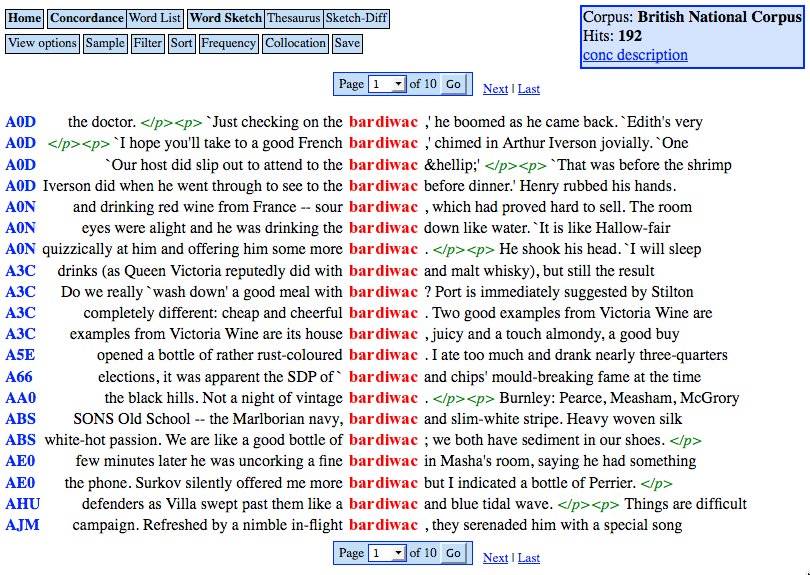
\includegraphics[width=10cm]{img/SE_bardiwac_conc}
  \end{center}
\end{frame}

\begin{frame}[c]
  \frametitle{Real-life concordance \& word sketch}
  \framesubtitle{http://beta.sketchengine.co.uk/}

  \begin{center}
    \ungap[1]
    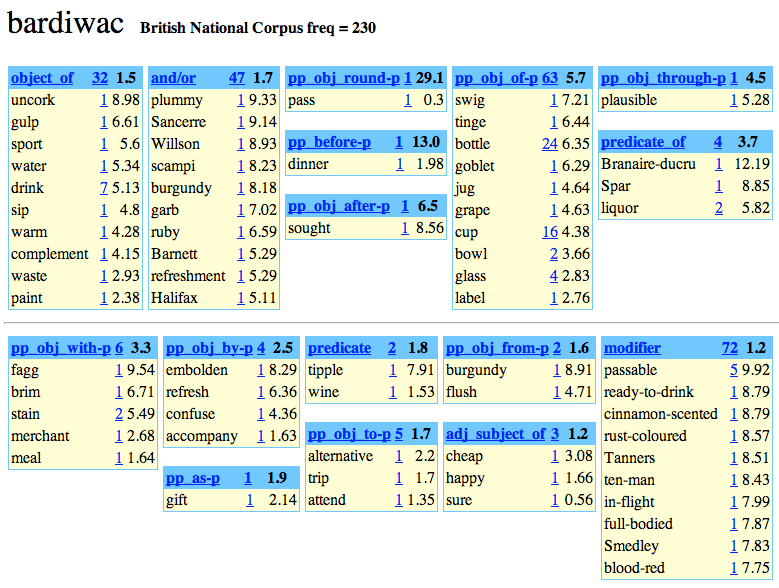
\includegraphics[width=10cm]{img/SE_bardiwac_sketch}
  \end{center}
\end{frame}

{\newcommand{\hg}[1]{\scriptsize\textpmhg{#1}}
\begin{frame}<beamer:1-4| handout:1-4>
  \frametitle{A thought experiment: deciphering hieroglyphs}
  % \framesubtitle{}

  \begin{center}
    \setlength{\arrayrulewidth}{1pt}
    \begin{tabular}{@{\rule{0mm}{1.2em} }lr*{6}{|c}|}
      && \hg{get} & \hg{sij} & \hg{ius} & \hg{hir} & \hg{iit} & \hg{kil} \\
      \hline
      \secondary<beamer:2| handout:2>{(knife)} & \secondary<beamer:2| handout:2>{\hg{naif}} & \secondary<beamer:2| handout:2>{51} & \secondary<beamer:2| handout:2>{20} & \secondary<beamer:2| handout:2>{84} &  \secondary<beamer:2| handout:2>{0} &  \secondary<beamer:2| handout:2>{3} &  \secondary<beamer:2| handout:2>{0} \\
      \hline
      \secondary<beamer:4| handout:4>{(cat)}   & \secondary<beamer:4| handout:4>{\hg{ket}}  &  \secondary<beamer:4| handout:4>{52} & \secondary<beamer:4| handout:4>{58} &  \secondary<beamer:4| handout:4>{4} &  \secondary<beamer:4| handout:4>{4} &  \secondary<beamer:4| handout:4>{6} & \secondary<beamer:4| handout:4>{26} \\
      \hline
      \h{???} & \h{\hg{dog}} & \primary{115} & \primary{83} & \primary{10} & \primary{42} & \primary{33} & \primary{17} \\
      \hline
      (boat)  & \hg{beut} &  59 & 39 & 23 &  4 &  0 &  0 \\
      \hline
      (cup)   & \hg{kap}  &  98 & 14 &  6 &  2 &  1 &  0 \\
      \hline
      \secondary<beamer:3| handout:3>{(pig)}  & \secondary<beamer:3| handout:3>{\hg{pigij}} &  \secondary<beamer:3| handout:3>{12} & \secondary<beamer:3| handout:3>{17} &  \secondary<beamer:3| handout:3>{3} &  \secondary<beamer:3| handout:3>{2} &  \secondary<beamer:3| handout:3>{9} & \secondary<beamer:3| handout:3>{27} \\
      \hline
      (banana) & \hg{nana} & 11 &  2 &  2 &  0 & 18 &  0 \\
      \hline
    \end{tabular}
    
    \gap[2]\Large
    \only<beamer:2| handout:2>{%
      sim(\primary{\hg{dog}}, \secondary{\hg{naif}}) = 0.770 }%
    \only<beamer:3| handout:3>{%
      sim(\primary{\hg{dog}}, \secondary{\hg{pigij}}) = 0.939 }%
    \only<beamer:4| handout:4>{%
      sim(\primary{\hg{dog}}, \secondary{\hg{ket}}) = 0.961 }%
  \end{center}

  \addnote{Similarity scores are cosine similarities on sparse log-scaled frequencies ($\log (f+1)$).}%
\end{frame}
}

{\newcommand{\hg}[1]{\scriptsize\textpmhg{#1}}
\begin{frame}
  \frametitle{English as seen by the computer \ldots}
  % \framesubtitle{}

  \begin{center}
    \ungap[1]
    \setlength{\arrayrulewidth}{1pt}
    \begin{tabular}{@{\rule{0mm}{1.2em} }l@{ }r*{6}{|c}|}
      && get & see & use & hear & eat & kill \\
      && \hg{get} & \hg{sij} & \hg{ius} & \hg{hir} & \hg{iit} & \hg{kil} \\
      \hline
      knife & \hg{naif} &  51 & 20 & 84 &  0 &  3 &  0 \\
      \hline
      cat   & \hg{ket}  &  52 & 58 &  4 &  4 &  6 & 26 \\
      \hline
      \h{dog} & \h{\hg{dog}} & \primary{115} & \primary{83} & \primary{10} & \primary{42} & \primary{33} & \primary{17} \\
      \hline
      boat  & \hg{beut} &  59 & 39 & 23 &  4 &  0 &  0 \\
      \hline
      cup   & \hg{kap}  &  98 & 14 &  6 &  2 &  1 &  0 \\
      \hline
      pig  & \hg{pigij} &  12 & 17 &  3 &  2 &  9 & 27 \\
      \hline
      banana & \hg{nana} & 11 &  2 &  2 &  0 & 18 &  0 \\
      \hline
    \end{tabular}
  \end{center}
  \hfill\light{\footnotesize verb-object counts from British National Corpus}
\end{frame}
}

\begin{frame}
  \frametitle{Geometric interpretation}
  % \framesubtitle{}

  \begin{columns}[T]
    \begin{column}{40mm}
      \begin{itemize}
      \item row vector \primary{$\vx_{\text{dog}}$} describes usage of word \emph{dog} in the corpus
      \item can be seen as coordinates of point in $n$-dimensional Euclidean space
       \end{itemize}
    \end{column}
    \begin{column}{75mm}      
      \gap[2]
      \begin{small}
        \setlength{\arrayrulewidth}{1pt}
        \begin{tabular}{r*{6}{|c}|}
          & get & see & use & hear & eat & kill \\
          \hline
          knife &  51 & 20 & 84 &  0 &  3 &  0 \\
          \hline
          cat  &  52 & 58 &  4 &  4 &  6 & 26 \\
          \hline
          \h{dog} & \primary{115} & \primary{83} & \primary{10} & \primary{42} & \primary{33} & \primary{17} \\
          \hline
          boat &  59 & 39 & 23 &  4 &  0 &  0 \\
          \hline
          cup  &  98 & 14 &  6 &  2 &  1 &  0 \\
          \hline
          pig  &  12 & 17 &  3 &  2 &  9 & 27 \\
          \hline
          banana & 11 &  2 &  2 &  0 & 18 &  0 \\
          \hline
        \end{tabular}
      \end{small}

      \begin{center}
        \h{co-occurrence matrix} $M$
      \end{center}
    \end{column}
  \end{columns}
\end{frame}

\begin{frame}
  \frametitle{Geometric interpretation}
  % \framesubtitle{}

  \begin{columns}[T]
    \begin{column}{40mm}
      \begin{itemize}
      \item row vector \primary{$\vx_{\text{dog}}$} describes usage of word \emph{dog} in the corpus
      \item can be seen as coordinates of point in $n$-dimensional Euclidean space
      \item illustrated for two dimensions:\\ \emph{get} and \emph{use}
      \item \primary{$\vx_{\text{dog}} = (115,10)$}
      \end{itemize}
    \end{column}
    \begin{column}{75mm}      
      \ungap[1]
      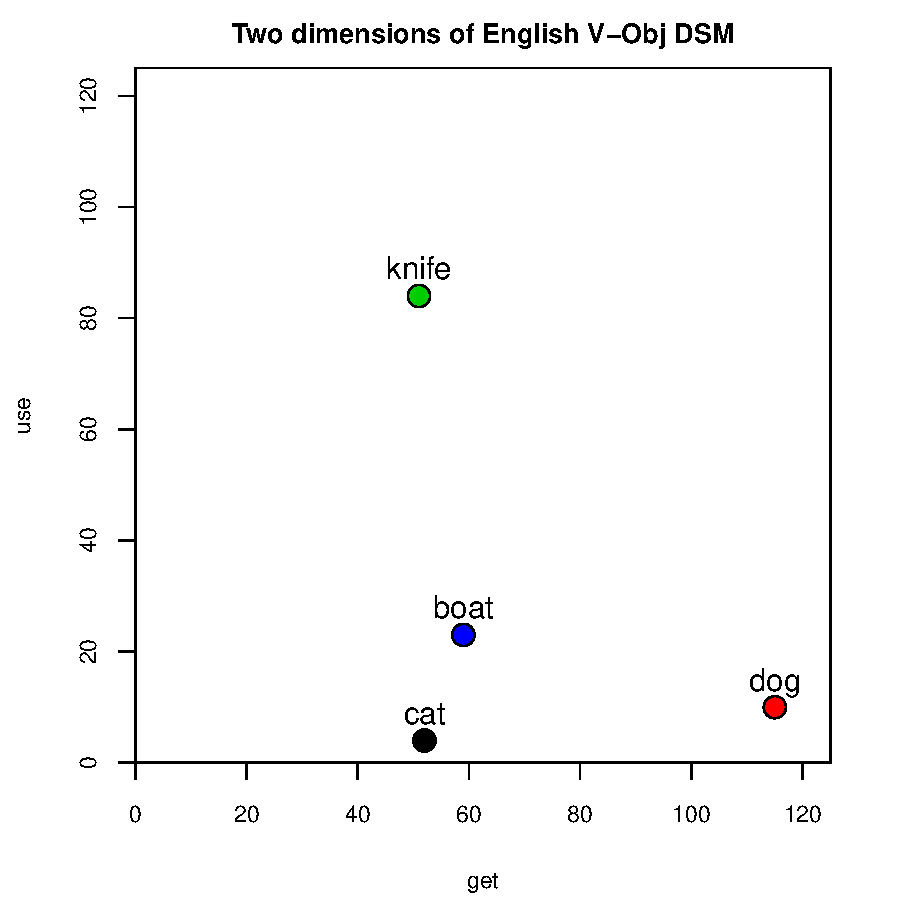
\includegraphics[width=75mm]{img/hieroglyph_2d_1}
    \end{column}
  \end{columns}
\end{frame}

\begin{frame}
  \frametitle{Geometric interpretation}
  % \framesubtitle{}

  \begin{columns}[T]
    \begin{column}{40mm}
      \begin{itemize}
      \item similarity = spatial proximity (Euclidean dist.)
      \item location depends on frequency of noun ($f_{\text{dog}} \approx 2.7\cdot f_{\text{cat}}$)
      \end{itemize}
    \end{column}
    \begin{column}{75mm}      
      \ungap[1]
      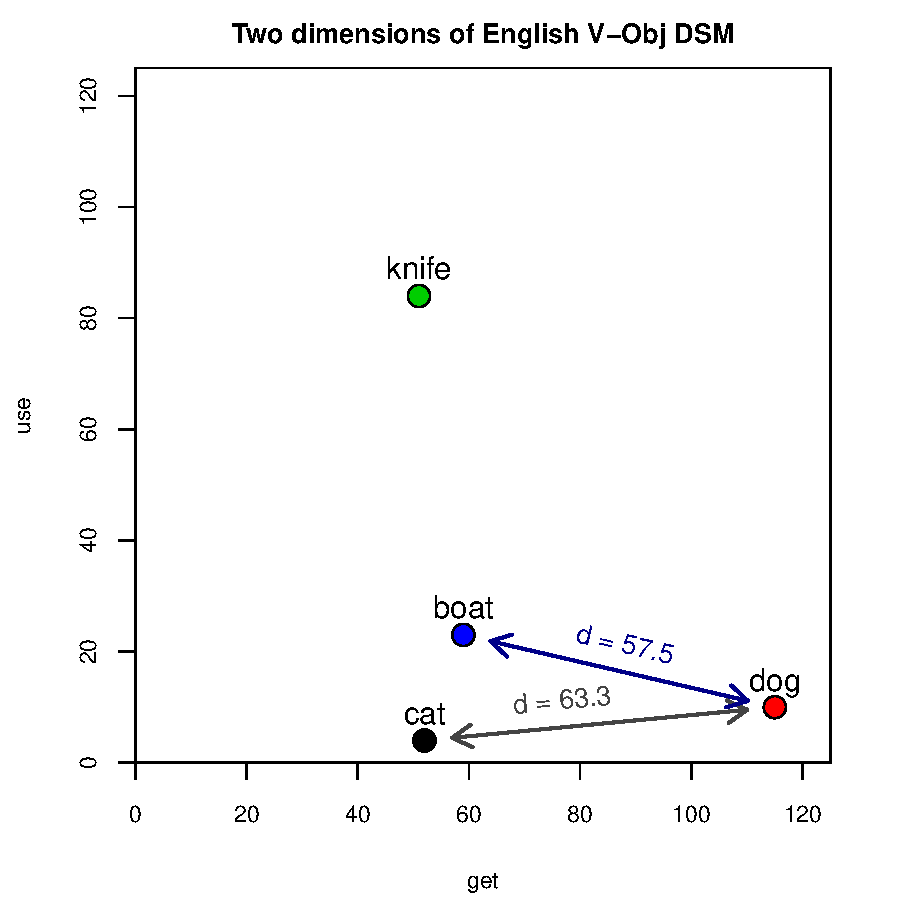
\includegraphics[width=75mm]{img/hieroglyph_2d_2}
    \end{column}
  \end{columns}
\end{frame}

\begin{frame}
  \frametitle{Geometric interpretation}
  % \framesubtitle{}

  \begin{columns}[T]
    \begin{column}{40mm}
      \begin{itemize}
      \item similarity = spatial proximity (Euclidean dist.)
      \item location depends on frequency of noun ($f_{\text{dog}} \approx 2.7\cdot f_{\text{cat}}$)
      \item direction more important than location
      \end{itemize}
    \end{column}
    \begin{column}{75mm}      
      \ungap[1]
      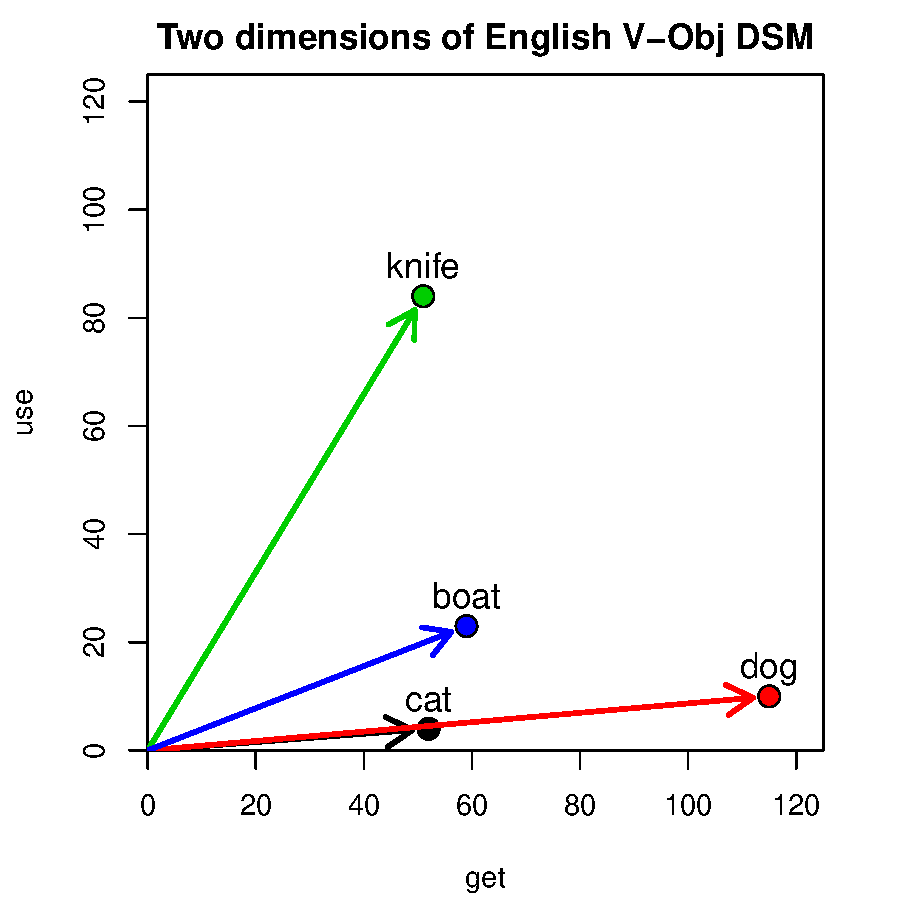
\includegraphics[width=75mm]{img/hieroglyph_2d_3}
    \end{column}
  \end{columns}
\end{frame}

\begin{frame}
  \frametitle{Geometric interpretation}
  % \framesubtitle{}

  \begin{columns}[T]
    \begin{column}{40mm}
      \begin{itemize}
      \item similarity = spatial proximity (Euclidean dist.)
      \item location depends on frequency of noun ($f_{\text{dog}} \approx 2.7\cdot f_{\text{cat}}$)
      \item direction more important than location
      \item<1-> normalise ``length'' $\norm{\vx_{\text{dog}}}$ of vector
      \item<2-> or use angle $\alpha$ as distance measure
      \end{itemize}
    \end{column}
    \begin{column}{75mm}
      \ungap[1]
      \only<beamer:1| handout:0>{%
        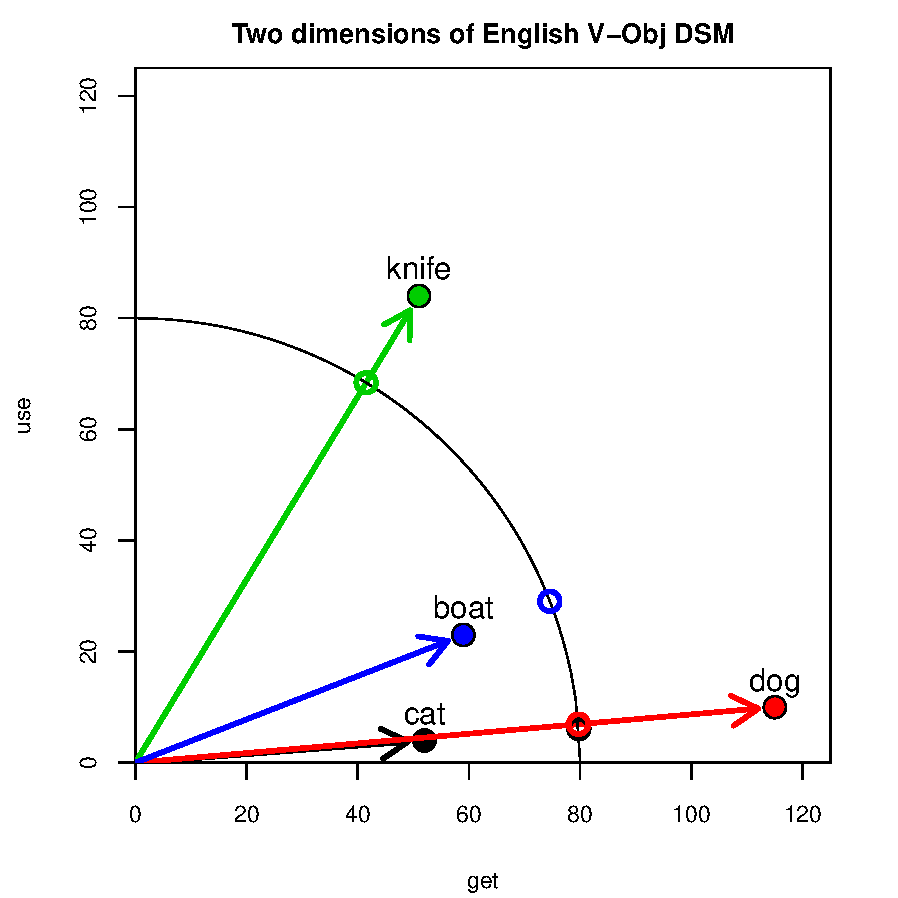
\includegraphics[width=75mm]{img/hieroglyph_2d_4}}%
      \only<beamer:2| handout:1>{%
        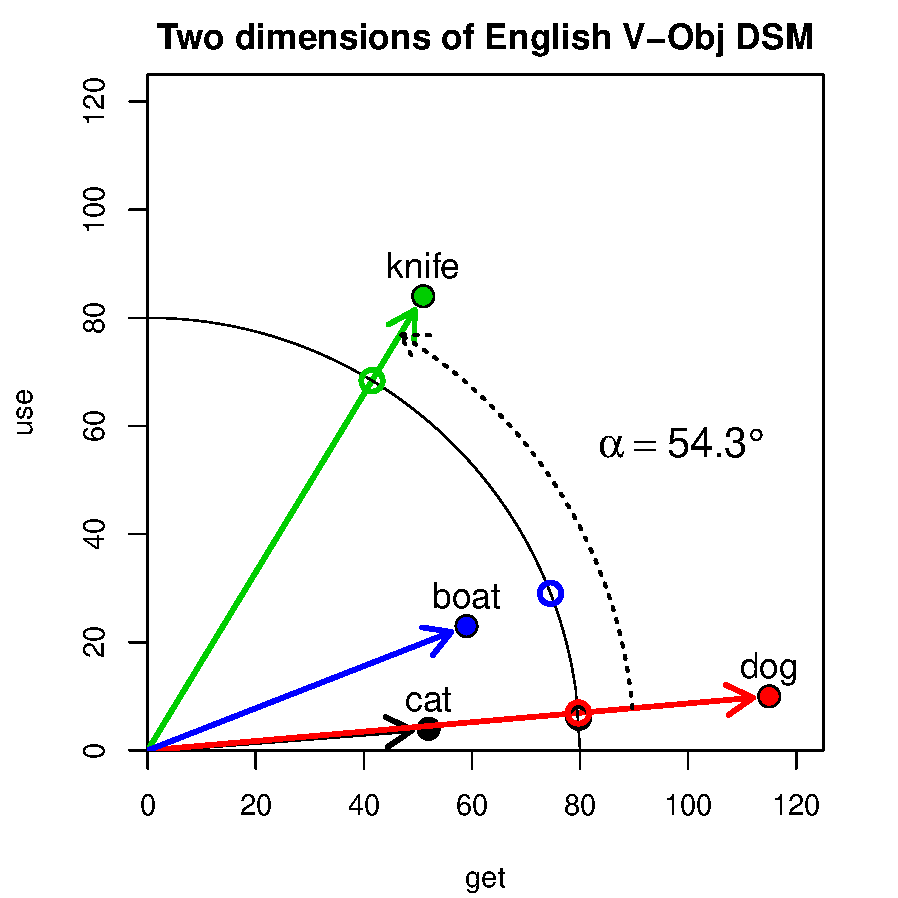
\includegraphics[width=75mm]{img/hieroglyph_2d_5}}%
    \end{column}
  \end{columns}
\end{frame}

\begin{frame}
  \frametitle{Semantic distances}
  % \framesubtitle{}

  \begin{columns}[T]
    \begin{column}{55mm}
      \begin{itemize}
      \item main result of distributional analysis are ``semantic'' distances between words
      \item typical applications
        \begin{itemize}
        \item nearest neighbours
        \item clustering of related words
        \item construct semantic map
        \end{itemize}
      \end{itemize}
    \end{column}
    \begin{column}{55mm}
      \ungap[1]
      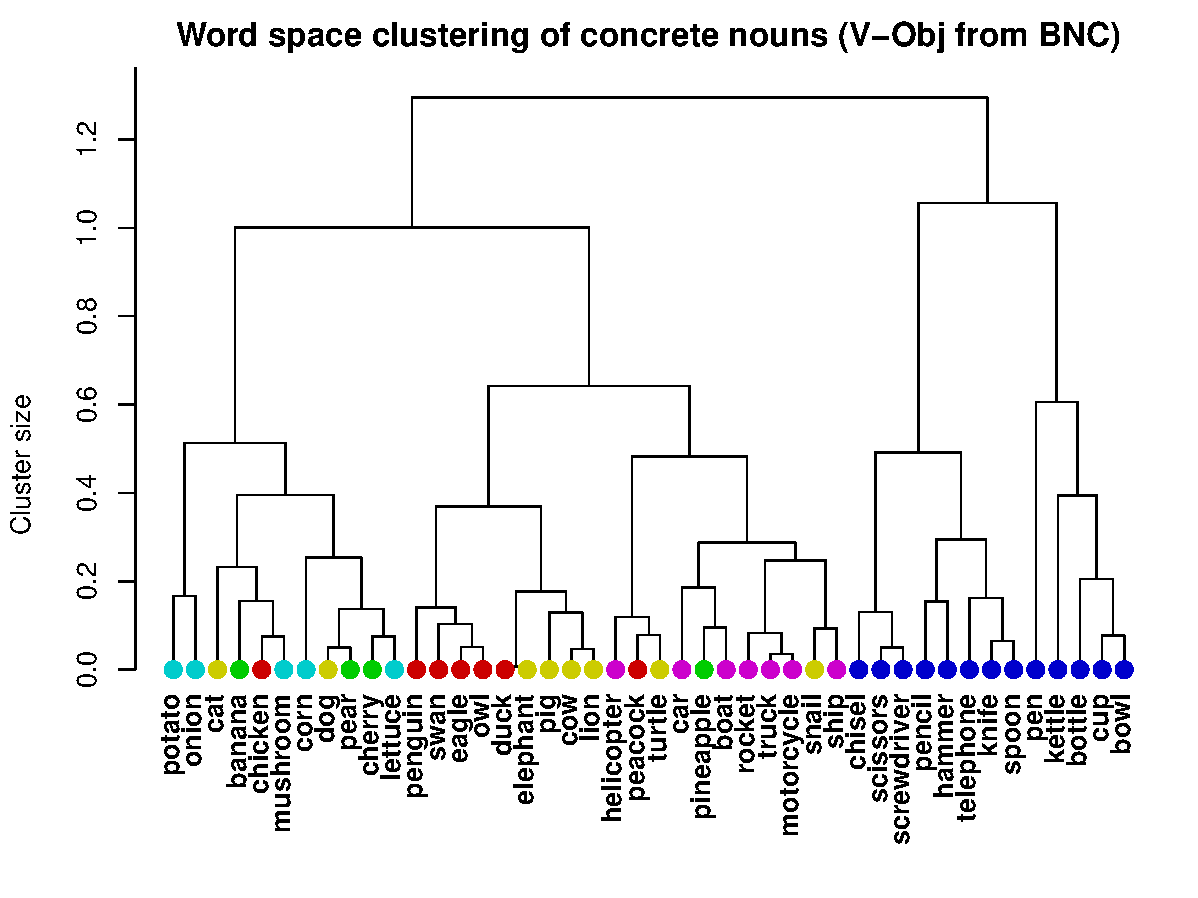
\includegraphics[width=50mm]{img/hieroglyph_clustering}

      \gap[1]
      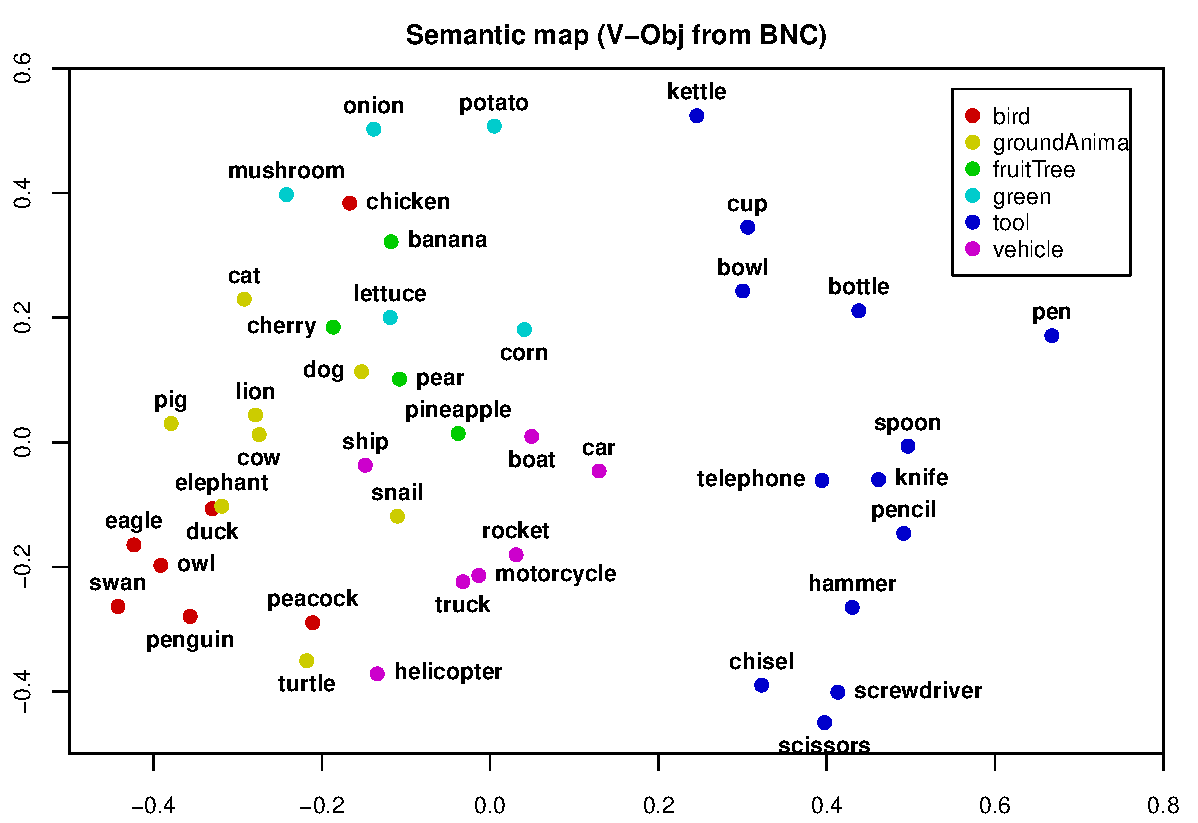
\includegraphics[width=50mm]{img/hieroglyph_semantic_map}
    \end{column}
  \end{columns}
\end{frame}

%%%%%%%%%%%%%%%%%%%%%%%%%%%%%%%%%%%%%%%%%%
\subsection{General overview}

\begin{frame}
  \frametitle{Tutorial overview}
  % \framesubtitle{}

  \TODO[Overview]
\end{frame}

\begin{frame}
  \frametitle{Further information}
  % \framesubtitle{}

  \begin{itemize}
  \item Handouts \& other materials vailable from homepage at
    \begin{center}
      \secondary{\url{http://wordspace.collocations.de/}}
    \end{center}
    \begin{itemize}
    \item[\hand] will be extended during the next few months
    \end{itemize}
  \item Tutorial is open source (CC), and can be downloaded from
    \begin{center}\footnotesize
      \secondary{\url{http://r-forge.r-project.org/projects/wordspace/}}
    \end{center}
  \item Compact DSM textbook in preparation for \primary{\emph{Synthesis Lectures on Human Language Technologies}} (Morgan \& Claypool)
  \end{itemize}

  \gap[1]
  \begin{center}
    \fbox{\parbox{7cm}{\centering
        This tutorial is based on joint work with Marco Baroni and Alessandro Lenci}}
  \end{center}
\end{frame}

\begin{frame}
  \frametitle{A very brief history of DSM}
  % \framesubtitle{}

  \begin{itemize}
  \item Introduced to computational linguistics in early 1990s
    following the probabilistic revolution \citep{Schuetze:92,Schuetze:98}
  \item Other early work in psychology \citep{Landauer:Dumais:97,Lund:Burgess:96}
    \begin{itemize}
    \item[\hand] influenced by Latent Semantic Indexing \citep{Dumais:etc:88} and efficient software implementations \citep{Berry:92}
    \end{itemize}
  \item<2-> Renewed interest in last few years
    \begin{itemize}
    \item<2-> \primary{2007}: CoSMo Workshop (at Context '07)
    \item<3-> \primary{2008}: ESSLLI Lexical Semantics Workshop \& Shared Task, Special Issue of the Italian Journal of Linguistics
    \item<4-> \primary{2009}: GeMS Workshop (EACL 2009), DiSCo Workshop (CogSci 2009), ESSLLI Advanced Course on DSM
    \item<5-> \primary{2010}: 2nd GeMS Workshop (ACL 2010), ESSLLI Workhsop on Compositionality \& DSM, Special Issue of JNLE (in prep.), Computational Neurolinguistics Workshop (NAACL-HLT 2010 --- \primary{don't miss it this Sunday!})
    \end{itemize}
  \end{itemize}
\end{frame}

\begin{frame}
  \frametitle{}
  % \framesubtitle{}

\end{frame}

%%%%%%%%%%%%%%%%%%%%%%%%%%%%%%%%%%%%%%%%%%
\subsection{}

\begin{frame}
  \frametitle{}
  % \framesubtitle{}

\end{frame}

%%%%%%%%%%%%%%%%%%%%%%%%%%%%%%%%%%%%%%%%%%
\subsection{}

\begin{frame}
  \frametitle{}
  % \framesubtitle{}

\end{frame}



\begin{frame}[fragile]
  \frametitle{}
  %% \framesubtitle{}

  % \ungap[1]
  \begin{alltt}
  \end{alltt}
\end{frame}

%%% Local Variables: 
%%% mode: latex
%%% TeX-master: "../workspace"
%%% End: 

%%%%%%%%%%%%%%%%%%%%%%%%%%%%%%%%%%%%%%%%%%%%%%%%%%%%%%%%%%%%%%%%%%%%%%
\section{Taxonomy of DSM parameters}

%%%%%%%%%%%%%%%%%%%%%%%%%%%%%%%%%%%%%%%%%%
\subsection{Definition \& overview}

\begin{frame}
  \frametitle{General definition of DSMs}
  % \framesubtitle{}

  \begin{block}{}
    A \h{distributional semantic model} (DSM) is a scaled and/or
    transformed co-occurrence matrix $\mathbf{M}$, such that each row $\vx$
    represents the distribution of a target term across contexts.
  \end{block}

  \begin{center}
    \begin{small}
      \setlength{\arrayrulewidth}{1pt}
      \begin{tabular}{r*{6}{|c}|}
        & get & see & use & hear & eat & kill \\
        \hline
        knife &  0.027 & -0.024 &  0.206 & -0.022 & -0.044 & -0.042 \\
        \hline
        cat   &  0.031 &  0.143 & -0.243 & -0.015 & -0.009 &  0.131 \\
        \hline
        \primary{dog}   & \primary{-0.026} &  \primary{0.021} & \primary{-0.212} &  \primary{0.064} &  \primary{0.013} &  \primary{0.014} \\
        \hline
        boat  & -0.022 &  0.009 & -0.044 & -0.040 & -0.074 & -0.042 \\
        \hline
        cup   & -0.014 & -0.173 & -0.249 & -0.099 & -0.119 & -0.042 \\
        \hline
        pig   & -0.069 &  0.094 & -0.158 &  0.000 &  0.094 &  0.265 \\
        \hline
        banana&  0.047 & -0.139 & -0.104 & -0.022 &  0.267 & -0.042 \\
        \hline
      \end{tabular}
    \end{small}
  \end{center}

  \hh{Term} = word, lemma, phrase, morpheme, \ldots
\end{frame}

\begin{frame}
  \frametitle{General definition of DSMs}
  % \framesubtitle{}

  Mathematical notation:
  \begin{itemize}
  \item $m \times n$ co-occurrence matrix $\mathbf{M}$ (example: $7\times 6$ matrix)
    \begin{itemize}
    \item $m$ rows = target terms
    \item $n$ columns = features or \hh{dimensions}
    \end{itemize}
    \begin{small}
      \gap[.5]
      \[
      \mathbf{M} =
      \begin{bmatrix}
        x_{11} & x_{12} & \cdots & x_{1n} \\
        x_{21} & x_{22} & \cdots & x_{2n} \\
        \vdots & \vdots & & \vdots \\
        x_{m1} & x_{m2} & \cdots & x_{mn}
      \end{bmatrix}
      \]
    \end{small}
  \item distribution vector $\vx_i$ = $i$-th row of $\mathbf{M}$, e.g.\ $\vx_3 = \vx_{\text{dog}}$
  \item components $\vx_i = (x_{i1}, x_{i2}, \ldots, x_{in})$ = features of $i$-th term:
    \begin{align*}
      \vx_3 &= (-0.026, 0.021, -0.212, 0.064, 0.013, 0.014) \\
      &= (x_{31}, x_{32}, x_{33}, x_{34}, x_{35}, x_{36})
    \end{align*}
  \end{itemize}

\end{frame}

\begin{frame}
  \frametitle{Overview of DSM parameters}
  % \framesubtitle{}

  \ungap[1]
  \begin{center}
    Linguistic pre-processing (definition of terms)\\
    \pause $\Downarrow$\\
    Term-context \vs\ term-term matrix\\
    \pause $\Downarrow$\\
    Size \& type of context / structured \vs\ unstructered\\
    \pause $\Downarrow$\\
    Geometric \vs\ probabilistic interpretation\\
    \pause $\Downarrow$\\
    Feature scaling\\
    \pause $\Downarrow$\\
    Normalisation of rows and/or columns\\
    \pause $\Downarrow$\\
    Similarity / distance measure\\
    \pause $\Downarrow$\\
    Compression
  \end{center}
\end{frame}

%%%%%%%%%%%%%%%%%%%%%%%%%%%%%%%%%%%%%%%%%%
\subsection{DSM parameters}

\begin{frame}
  \frametitle{Corpus pre-processing}
  \begin{itemize}
  \item Minimally, corpus must be tokenised \so identify terms
  \item Linguistic annotation
    \begin{itemize}
    \item part-of-speech tagging
    \item lemmatisation / stemming
    \item word sense disambiguation (rare)
    \item shallow syntactic patterns
    \item dependency parsing
    \end{itemize}
    \pause
  \item Generalisation of terms
    \begin{itemize}
    \item often lemmatised to reduce data sparseness:\\
      \emph{go, goes, went, gone, going} \so \emph{go}
    \item POS disambiguation (\emph{light}/N \vs\ \emph{light}/A \vs\ \emph{light}/V)
    \item word sense disambiguation (\emph{bank}\tsub{river} \vs\ \emph{bank}\tsub{finance})
    \end{itemize}
  \pause
  \item Trade-off between deeper linguistic analysis and
    \begin{itemize}
    \item need for language-specific resources
    \item possible errors introduced at each stage of the analysis
    \item even more parameters to optimise / cognitive plausibility
    \end{itemize}
  \end{itemize}
\end{frame}

\begin{frame}
  \frametitle{Effects of pre-processing}
  \framesubtitle{}

  \centering
  Nearest neighbours of \emph{walk} (BNC)
  \footnotesize
  \begin{columns}[t]
    \column{4cm}
    \begin{block}{word forms}
      \begin{itemize}
      \item stroll
      \item walking
      \item walked
      \item go
      \item path
      \item drive
      \item ride
      \item wander
      \item sprinted
      \item sauntered
      \end{itemize}
    \end{block}
    \column{4cm}
    \begin{block}{lemmatised corpus}
      \begin{itemize}
      \item hurry
      \item stroll
      \item stride
      \item trudge
      \item amble
      \item wander
      \item walk-nn
      \item walking
      \item retrace
      \item scuttle 
      \end{itemize}
    \end{block}
  \end{columns}
\end{frame}

\begin{frame}
  \frametitle{Effects of pre-processing}

  \centering
  Nearest neighbours of \emph{arrivare} (Repubblica)
  \footnotesize
  \begin{columns}[t]
    \column{4cm}
    \begin{block}{word forms}
      \begin{itemize}
      \item  giungere
      \item  \counterpoint{raggiungere}
      \item  \primary{arrivi}
      \item  raggiungimento
      \item  \counterpoint{raggiunto}
      \item  trovare
      \item  \counterpoint{raggiunge}
      \item  \primary{arrivasse}
      \item  \primary{arriver\`a}
      \item  concludere
      \end{itemize}
    \end{block}
    \column{4cm}
    \begin{block}{lemmatised corpus}
      \begin{itemize}
      \item giungere
      \item aspettare
      \item attendere
      \item arrivo-nn
      \item ricevere
      \item accontentare
      \item approdare
      \item pervenire
      \item venire
      \item piombare
      \end{itemize}
    \end{block}
  \end{columns}
  \addnote{Colours seem to indicate inflected forms belonging to the same lemma.}%
\end{frame}

\begin{frame}
  \frametitle{Overview of DSM parameters}
  % \framesubtitle{}

  \ungap[1]
  \begin{center}
    Linguistic pre-processing (definition of terms)\\
    $\Downarrow$\\
    \h{Term-context \vs\ term-term matrix}\\
    $\Downarrow$\\
    Size \& type of context / structured \vs\ unstructered\\
    $\Downarrow$\\
    Geometric \vs\ probabilistic interpretation\\
    $\Downarrow$\\
    Feature scaling\\
    $\Downarrow$\\
    Normalisation of rows and/or columns\\
    $\Downarrow$\\
    Similarity / distance measure\\
    $\Downarrow$\\
    Compression
  \end{center}
\end{frame}

\begin{frame}
  \frametitle{Term-context \vs\ term-term matrix}
  % \framesubtitle{}

  \h{Term-context matrix} records frequency of term in each individual context (typically a sentence or document)
  \begin{center}
    \begin{tabular}{l|c|c|c|c}
      & doc$_1$ & doc$_2$ & doc$_3$ & $\cdots$ \\
      \hline
      boat & 1 & 3 & 0 & $\cdots$ \\
      \hline
      cat  & 0 & 0 & 2 & $\cdots$ \\
      \hline
      dog  & 1 & 0 & 1 & $\cdots$ \\
      \hline
    \end{tabular}
  \end{center}
  
  \begin{itemize}
  \item Typical contexts are non-overlapping textual units (Web page, encyclopaedia article, paragraph, sentence, \ldots)
  \item<2-> Contexts can also be generalised, e.g.
    \begin{itemize}
    \item bag of content words
    \item specific pattern of POS tags
    \item subcategorisation pattern of target verb
    \end{itemize}
  \item<2-> Term-context matrix is usually very \h{sparse}
  \end{itemize}
\end{frame}

\begin{frame}
  \frametitle{Term-context \vs\ term-term matrix}
  % \framesubtitle{}

  \h{Term-term matrix} records co-occurrence frequencies of context terms for each target term (often target terms $\neq$ context terms)
  \begin{center}
    \begin{tabular}{l|c|c|c|c}
      & see & use & hear & $\cdots$ \\
      \hline
      boat & 39 & 23 & 4 & $\cdots$ \\
      \hline
      cat  & 58 & 4 & 4 & $\cdots$ \\
      \hline
      dog  & 83 & 10 & 42 & $\cdots$ \\
      \hline
    \end{tabular}
  \end{center}
  
  \begin{itemize}
  \item<2-> Different types of contexts \citep{Evert:08}
    \begin{itemize}
    \item \hh{surface context} (word or character window)
    \item \hh{textual context} (non-overlapping segments)
    \item \hh{syntactic contxt} (specific syntagmatic relation)
    \end{itemize}
  \item<2-> Can be seen as smoothing of term-context matrix
    \begin{itemize}
    \item average over similar contexts (with same context terms)
    \item data sparseness reduced, except for small windows
    \end{itemize}
  \end{itemize}
\end{frame}

\begin{frame}
  \frametitle{Overview of DSM parameters}
  % \framesubtitle{}

  \ungap[1]
  \begin{center}
    Linguistic pre-processing (definition of terms)\\
    $\Downarrow$\\
    Term-context \vs\ term-term matrix\\
    $\Downarrow$\\
    \h{Size \& type of context / structured \vs\ unstructered}\\
    $\Downarrow$\\
    Geometric \vs\ probabilistic interpretation\\
    $\Downarrow$\\
    Feature scaling\\
    $\Downarrow$\\
    Normalisation of rows and/or columns\\
    $\Downarrow$\\
    Similarity / distance measure\\
    $\Downarrow$\\
    Compression
  \end{center}
\end{frame}

\begin{frame}
  \frametitle{Surface context}
  
  \begin{center}
    Context term occurs \primary{within a window of $k$ words} around target.
  \end{center}

  The {\color{secondary}silhouette of the} \primary{sun}
  {\color{secondary}beyond a wide-open} bay on {\color{secondary}the lake;
    the} \primary{sun} {\color{secondary}still glitters although} evening
  has arrived in Kuhmo. It's midsummer; the living room has its
  instruments and other objects in each of its corners.
  
  \gap
  Parameters:
  \begin{itemize}
  \item window size (in words or characters)
  \item symmetric \vs\ one-sided window
  \item uniform or ``triangular'' (distance-based) weighting
  \item window clamped to sentences or other textual units?
  \end{itemize}
\end{frame}


\begin{frame}
  \frametitle{Effect of different window sizes}
  \framesubtitle{}

  \centering
  Nearest neighbours of \emph{dog} (BNC)
  \footnotesize
  \begin{columns}[t]
    \column{4cm}
    \begin{block}{2-word window}
      \begin{itemize}
      \item cat
      \item horse
      \item fox
      \item pet
      \item rabbit
      \item pig
      \item animal
      \item mongrel
      \item sheep
      \item pigeon
      \end{itemize}
    \end{block}
    \column{4cm}
    \begin{block}{30-word window}
      \begin{itemize}
      \item kennel
      \item puppy
      \item pet
      \item bitch
      \item terrier
      \item rottweiler
      \item canine
      \item cat
      \item to bark
      \item Alsatian
      \end{itemize}
    \end{block}
  \end{columns}
\end{frame}


\begin{frame}
  \frametitle{Textual context}
  
  \begin{center}
    Context term is in the \primary{same linguistic unit} as target.
  \end{center}

  {\color{secondary}The silhouette of the} \primary{sun}
  {\color{secondary}beyond a wide-open bay on the lake; the}
  \primary{sun} {\color{secondary}still glitters although evening has
    arrived in Kuhmo.} It's midsummer; the living room has its
  instruments and other objects in each of its corners.
  
  \gap
  Parameters:
  \begin{itemize}
  \item type of linguistic unit
    \begin{itemize}
    \item sentence
    \item paragraph
    \item turn in a conversation
    \item Web page
    \end{itemize}
  \end{itemize}
\end{frame}

\begin{frame}
  \frametitle{Syntactic context}
  
  \ungap
  \begin{center}
    Context term is linked to target by a \primary{syntactic dependency}\\
    (e.g. subject, modifier, \ldots).
  \end{center}

  The {\color{secondary}silhouette} of the \primary{sun} beyond a
  wide-open {\color{secondary}bay} on the lake; the \primary{sun}
  still {\color{secondary}glitters} although evening has arrived in
  Kuhmo. It's midsummer; the living room has its instruments and other
  objects in each of its corners.
  
  \gap
  Parameters:
  \begin{itemize}
  \item types of syntactic dependency \citep{Pado:Lapata:07}
  \item direct \vs\ indirect dependency paths
    \begin{itemize}
    \item direct dependencies
    \item direct + indirect dependencies
    \end{itemize}
  \item homogeneous data (e.g.\ only verb-object) \vs\\
    heterogeneous data (e.g.\ all children and parents of the verb)
  \item maximal length of dependency path
  \end{itemize}
\end{frame}


\begin{frame}
  \frametitle{``Knowledge pattern'' context}
  
  \begin{center}
    Context term is linked to target by a \primary{lexico-syntactic pattern}\\
    (text mining, cf.\ Hearst 1992, Pantel \& Pennacchiotti 2008, etc.).
  \end{center}  

  In Provence, Van Gogh painted with bright \primary{colors}
  {\color{counterpoint}such as} {\color{secondary}red} {\color{counterpoint}and}
  {\color{secondary}yellow}.  These \primary{colors}
  {\color{counterpoint}produce} incredible {\color{secondary}effects} on
  anybody looking at his paintings.
  
  \gap
  Parameters:
  \begin{itemize}
  \item inventory of lexical patterns
    \begin{itemize}
    \item lots of research to identify semantically interesting patterns (cf. Almuhareb \& Poesio 2004,
      Veale \& Hao 2008, etc.)
    \end{itemize}
  \item fixed \vs\ flexible patterns
    \begin{itemize}
    \item patterns are mined from large corpora and automatically generalised (optional elements, POS tags or semantic classes)
    \end{itemize}
  \end{itemize}
\end{frame}

\begin{frame}[c]
  \frametitle{Structured vs.\ unstructured context}
  % \framesubtitle{}

  \begin{itemize}
  \item In \h{unstructered} models, context specification acts as a \hh{filter}
    \begin{itemize}
    \item determines whether context tokens counts as co-occurrence
    \item e.g.\ linked by specific syntactic relation such as verb-object
    \item[]
    \end{itemize}
    \pause
  \item In \h{structured} models, context words are \hh{subtyped}
    \begin{itemize}
    \item depending on their position in the context
    \item e.g.\ left \vs\ right context, type of syntactic relation, etc.
    \end{itemize}
  \end{itemize}
\end{frame}

\begin{frame}
  \frametitle{Structured \vs\ unstructured surface context}

  A dog bites a man. The man's dog bites a dog.  A dog bites a man.
  
 \begin{center}
    \begin{tabular}{r|c}
      \h{unstructured} &  bite \\
      dog & 4 \\
      man & 3 
    \end{tabular}
  \end{center}

  \gap[2]\pause
  A dog bites a man. The man's dog bites a dog.  A dog bites a man.
  
  \begin{center}
    \begin{tabular}{r|c|c}
      \h{structured} &  bite-l & bite-r \\
      dog & 3 & 1 \\
      man & 1  & 2
    \end{tabular}
  \end{center}
\end{frame}


\begin{frame}
  \frametitle{Structured \vs\ unstructured dependency context}

  A dog bites a man. The man's dog bites a dog.  A dog bites a man.
  
  \begin{center}
    \begin{tabular}{r|c}
      \h{unstructured} &  bite \\
      dog & 4 \\
      man & 2 
    \end{tabular}
  \end{center}

  \gap[2]\pause
  A dog bites a man. The man's dog bites a dog.  A dog bites a man.
  
   \begin{center}
     \begin{tabular}{r|c|c}
       \h{structured} &  bite-subj & bite-obj \\
       dog & 3 & 1 \\
       man & 0  & 2
     \end{tabular}
   \end{center}
\end{frame}


\begin{frame}
  \frametitle{Comparison}

  \begin{itemize}
  \item Unstructured context
    \begin{itemize}
    \item data less sparse (e.g.\ \emph{man kills} and \emph{kills man} both
      map to the \emph{kill} dimension of the vector $\vx_{\text{man}}$)
    \item[]
    \end{itemize}
  \item Structured context
    \begin{itemize}
    \item more sensitive to semantic distinctions\\
      (\emph{kill-subj} and \emph{kill-obj} are rather different
      things!)
    \item dependency relations provide a form of syntactic ``typing''
      of the DSM dimensions (the ``subject'' dimensions, the
      ``recipient'' dimensions, etc.)
     \item important to account for word-order and compositionality 
    \end{itemize}
  \end{itemize}
\end{frame}

\begin{frame}
  \frametitle{Overview of DSM parameters}
  % \framesubtitle{}

  \ungap[1]
  \begin{center}
    Linguistic pre-processing (definition of terms)\\
    $\Downarrow$\\
    Term-context \vs\ term-term matrix\\
    $\Downarrow$\\
    Size \& type of context / structured \vs\ unstructered\\
    $\Downarrow$\\
    \h{Geometric \vs\ probabilistic interpretation}\\
    $\Downarrow$\\
    Feature scaling\\
    $\Downarrow$\\
    Normalisation of rows and/or columns\\
    $\Downarrow$\\
    Similarity / distance measure\\
    $\Downarrow$\\
    Compression
  \end{center}
\end{frame}


\begin{frame}
  \frametitle{Geometric vs.\ probabilistic interpretation}
  % \framesubtitle{}

  \begin{itemize}
  \item Geometric interpretation
    \begin{itemize}
    \item row vectors as points or arrows in $n$-dim.\ space
    \item very intuitive, good for visualisation
    \item use techniques from geometry and linear algebra
    \item[]
    \end{itemize}
    \pause
  \item Probabilistic interpretation
    \begin{itemize}
    \item co-occurrence matrix as observed sample statistic
    \item ``explained'' by generative probabilistic model
    \item recent work focuses on hierarchical Bayesian models
    \item probabilistic LSA \citep{Hoffmann:99}, Latent Semantic
      Clustering \citep{Rooth:etc:99}, Latent Dirichlet Allocation
      \citep{Blei:Ng:Jordan:03}, etc.
    \item explicitly accounts for random variation of frequency counts
    \item intuitive and plausible as topic model
    \item[]
    \end{itemize}
    \pause
  \item[\hand] focus exclusively on geometric interpretation in this tutorial
  \end{itemize}
\end{frame}

\begin{frame}
  \frametitle{Overview of DSM parameters}
  % \framesubtitle{}

  \ungap[1]
  \begin{center}
    Linguistic pre-processing (definition of terms)\\
    $\Downarrow$\\
    Term-context \vs\ term-term matrix\\
    $\Downarrow$\\
    Size \& type of context / structured \vs\ unstructered\\
    $\Downarrow$\\
    Geometric \vs\ probabilistic interpretation\\
    $\Downarrow$\\
    \h{Feature scaling}\\
    $\Downarrow$\\
    Normalisation of rows and/or columns\\
    $\Downarrow$\\
    Similarity / distance measure\\
    $\Downarrow$\\
    Compression
  \end{center}
\end{frame}

\begin{frame}
  \frametitle{Feature scaling}

  Feature scaling is used to ``discount'' less important features:
  \begin{itemize}
  \item<1-> Logarithmic scaling: $x' = \log (x+1)$\\
    (cf.\ Weber-Fechner law for human perception)
  \item<2-> Relevance weighting, e.g.\ \primary{tf.idf} (information retrieval)
  \item<3-> Statistical \h{association measures} \citep{Evert:04phd,Evert:08}
    take frequency of target word and context feature into account
    \begin{itemize}
    \item the less frequent the target word and (more importantly) the
      context feature are, the higher the weight given to their
      observed co-occurrence count should be (because their expected
      chance co-occurrence frequency is low)
    \item different measures -- e.g., mutual information,
      log-likelihood ratio -- differ in how they balance observed and
      expected co-occurrence frequencies
    \end{itemize}
  \end{itemize}
\end{frame}

\begin{frame}
  \frametitle{Association measures: Mutual Information (MI)}

  \begin{center}
    \begin{tabular}{llrrr}
      word\tsub1 & word\tsub2 & $f_{\text{obs}}$ & $f_1$ & $f_2$ \\
      \hline
      dog & small & 855 &33,338 & 490,580\\ 
      dog & domesticated & 29 &33,338& 918\\
    \end{tabular}
  \end{center}

  \pause
  Expected co-occurrence frequency:
  \[
  f_{\text{exp}} = \frac{f_1 \cdot f_2}{N}
  \]
  
  \pause
  Mutual Information compares observed \vs\ expected frequency:
  \[
  \text{MI}(w_{1},w_{2}) =
  \log_{2} \frac{f_{\text{obs}}}{f_{\text{exp}}} =
  \log_2 \frac{N\cdot f_{\text{obs}}}{f_1\cdot f_2}
  \]
  
  \pause
  Disadvantage: MI overrates combinations of rare terms.
\end{frame}



\begin{frame}
  \frametitle{Other association measures}

  Log-likelihood ratio \citep{Dunning:93} has more complex form, but
  its ``core'' is known as local MI \citep{Evert:04phd}.

  \[
  \text{local-MI}(w_1, w_2) = f_{\text{obs}} \cdot \text{MI}(w_1, w_2)
  \]
 
  \pause
  \begin{center}
    \begin{tabular}{llrrr}
      word\tsub1 & word\tsub2 & $f_{\text{obs}}$ & MI & local-MI \\
      \hline
      dog & small & 855 & 3.96 & 3382.87\\ 
      dog & domesticated & 29  & 6.85 & 198.76\\
      dog & sgjkj & 1 & 10.31 &  10.31\\ 
    \end{tabular}
  \end{center}

  \pause
  The t-score measure \citep{Church:Hanks:90} is popular in lexicography:
  \[
  \text{t-score}(w_1, w_2) = \frac{f_{\text{obs}} - f_{\text{exp}}}{\sqrt{f_{\text{obs}}}}
  \]

  Details \& many more measures: \secondary{\url{http://www.collocations.de/}}
\end{frame}


\begin{frame}
  \frametitle{Overview of DSM parameters}
  % \framesubtitle{}

  \ungap[1]
  \begin{center}
    Linguistic pre-processing (definition of terms)\\
    $\Downarrow$\\
    Term-context \vs\ term-term matrix\\
    $\Downarrow$\\
    Size \& type of context / structured \vs\ unstructered\\
    $\Downarrow$\\
    Geometric \vs\ probabilistic interpretation\\
    $\Downarrow$\\
    Feature scaling\\
    $\Downarrow$\\
    \h{Normalisation of rows and/or columns}\\
    $\Downarrow$\\
    Similarity / distance measure\\
    $\Downarrow$\\
    Compression
  \end{center}
\end{frame}

\begin{frame}[c]
  \frametitle{Normalisation of row vectors}
  % \framesubtitle{}
  
  \begin{columns}[c]
    \begin{column}{5cm}
      \begin{itemize}
      \item geometric distances only make sense if vectors are normalised to unit length
      \item divide vector by its length: \[ \vx / \norm{\vx} \]
      \item normalisation depends on distance measure!
      \item special case: scale to relative frequencies with
        $\norm[1]{\vx} = \abs{x_1} + \dots + \abs{x_n}$
      \end{itemize}
    \end{column}
    \begin{column}{6cm}
      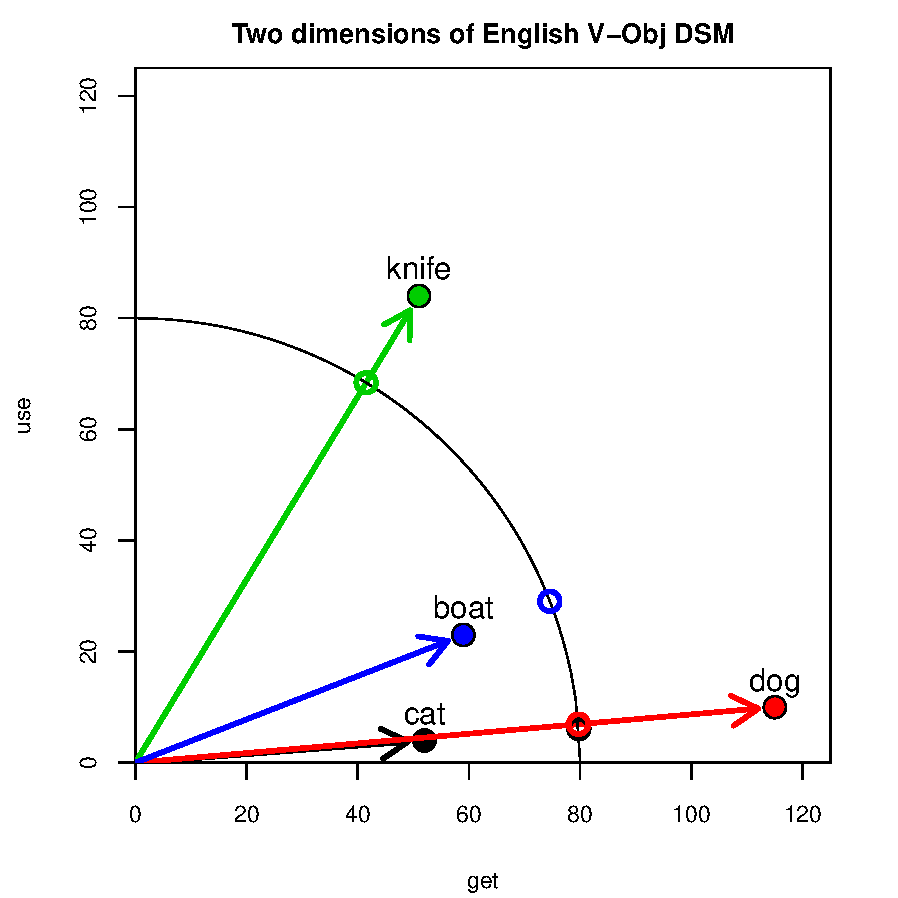
\includegraphics[width=6cm]{img/hieroglyph_2d_4}
    \end{column}
  \end{columns}
\end{frame}

\begin{frame}
  \frametitle{Scaling of column vectors}
  % \framesubtitle{}

  \begin{itemize}
  \item In statistical analysis and machine learning, features are
    usually \primary{centred} and \primary{scaled} so that
    \begin{align*}
      \text{mean} & \quad \mu = 0 \\
      \text{variance} & \quad \sigma^2 = 1
    \end{align*}
  \item In DSM research, this step is less common for columns of $\mathbf{M}$
    \begin{itemize}
    \item centring is a prerequisite for certain dimensionality
      reduction and data analysis techniques (esp.\ PCA)
    \item scaling may give too much weight to rare features
    \end{itemize}
    \pause
  \item $\mathbf{M}$ cannot be row-normalised and column-scaled at the
    same time (result depends on ordering of the two steps)
  \end{itemize}
\end{frame}

\begin{frame}
  \frametitle{Overview of DSM parameters}
  % \framesubtitle{}

  \ungap[1]
  \begin{center}
    Linguistic pre-processing (definition of terms)\\
    $\Downarrow$\\
    Term-context \vs\ term-term matrix\\
    $\Downarrow$\\
    Size \& type of context / structured \vs\ unstructered\\
    $\Downarrow$\\
    Geometric \vs\ probabilistic interpretation\\
    $\Downarrow$\\
    Feature scaling\\
    $\Downarrow$\\
    Normalisation of rows and/or columns\\
    $\Downarrow$\\
    \h{Similarity / distance measure}\\
    $\Downarrow$\\
    Compression
  \end{center}
\end{frame}

\begin{frame}
  \frametitle{Geometric distance}
  %% \framesubtitle{}

  \begin{columns}[T]
    \begin{column}{60mm}
      \begin{itemize}
      \item \h{Distance} between vectors $\vu, \vv \in \setR^n$ \so
        (dis)\h{similarity}
        \begin{itemize}
        \item $\vu = (u_1, \ldots, u_n)$
        \item $\vv = (v_1, \ldots, v_n)$
        \end{itemize}
      \item<2-> \h{Euclidean} distance $\dist[2]{\vu}{\vv}$
      \item<3-> ``City block'' \h{Manhattan} distance $\dist[1]{\vu}{\vv}$
      \item<4-> Both are special cases of the \h{Minkowski} $p$-distance
        $\dist[p]{\vu}{\vv}$ (for $p\in [1, \infty]$)
      \end{itemize}
    \end{column}
    \begin{column}{45mm}
      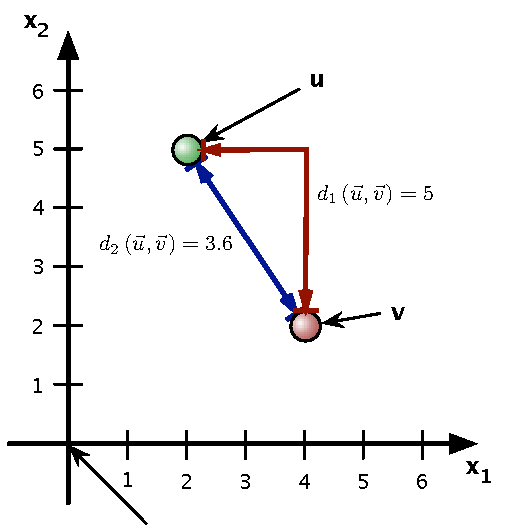
\includegraphics[width=45mm]{img/2_distance_examples}
    \end{column}
  \end{columns}
  \gap[.5]
  \only<beamer:2| handout:0>{%
    \[ \dist[2]{\vu}{\vv} \coloneq \sqrt{(u_1 - v_1)^2 + \dots + (u_n - v_n)^2} \] }
  \only<beamer:3| handout:0>{%
    \[ \dist[1]{\vu}{\vv} \coloneq \abs{u_1 - v_1} + \dots + \abs{u_n - v_n} \] }
  \only<beamer:4-| handout:1>{%
    \[ \dist[p]{\vu}{\vv} \coloneq \bigl(
    \abs{u_1 - v_1}^p + \dots + \abs{u_n - v_n}^p
    \bigr)^{1/p} \] }
  \only<beamer:5-| handout:1>{%
    \[ \dist[\infty]{\vu}{\vv} = \max \bigset{\abs{u_1 - v_1}, \ldots, \abs{u_n - v_n}} \] }
\end{frame}


\begin{frame}
  \frametitle{Other distance measures}
  % \framesubtitle{}
  
  \begin{itemize}
  \item Information theory: \h{Kullback-Leibler} (KL) \h{divergence} for probability vectors (non-negative, $\norm[1]{\vx} = 1$)
    \[
    \KL{\vu}{\vv} = \sum_{i=1}^n u_i \cdot \log_2 \frac{u_i}{v_i}
    \]
    \pause
  \item Properties of KL divergence
    \begin{itemize}
    \item most appropriate in a probabilistic interpretation of $\mathbf{M}$
    \item not symmetric, unlike all other measures
    \item alternatives: skew divergence, Jensen-Shannon divergence
    \end{itemize}
  \end{itemize}
\end{frame}

\begin{frame}
  \frametitle{Similarity measures}
  % \framesubtitle{}
  
  \begin{columns}[c]
    \begin{column}{5cm}
      \begin{itemize}
        \item angle $\alpha$ between two vectors $\vu,\vv$ is given by
          \begin{align*}
            \cos \alpha &= 
            \frac{\sum_{i=1}^n u_i\cdot v_i}{
              \sqrt{\sum_i u_i^2}\cdot \sqrt{\sum_i v_i^2}}
            \\
            &= \frac{\sprod{\vu}{\vv}}{\norm[2]{\vu}\cdot \norm[2]{\vv}}
        \end{align*}
      \item<2-> \h{cosine} measure of similarity: $\cos \alpha$
        \begin{itemize}
        \item $\cos \alpha = 1$ \so collinear
        \item $\cos \alpha = 0$ \so orthogonal
        \end{itemize}
      \end{itemize}
    \end{column}
    \begin{column}{6cm}
      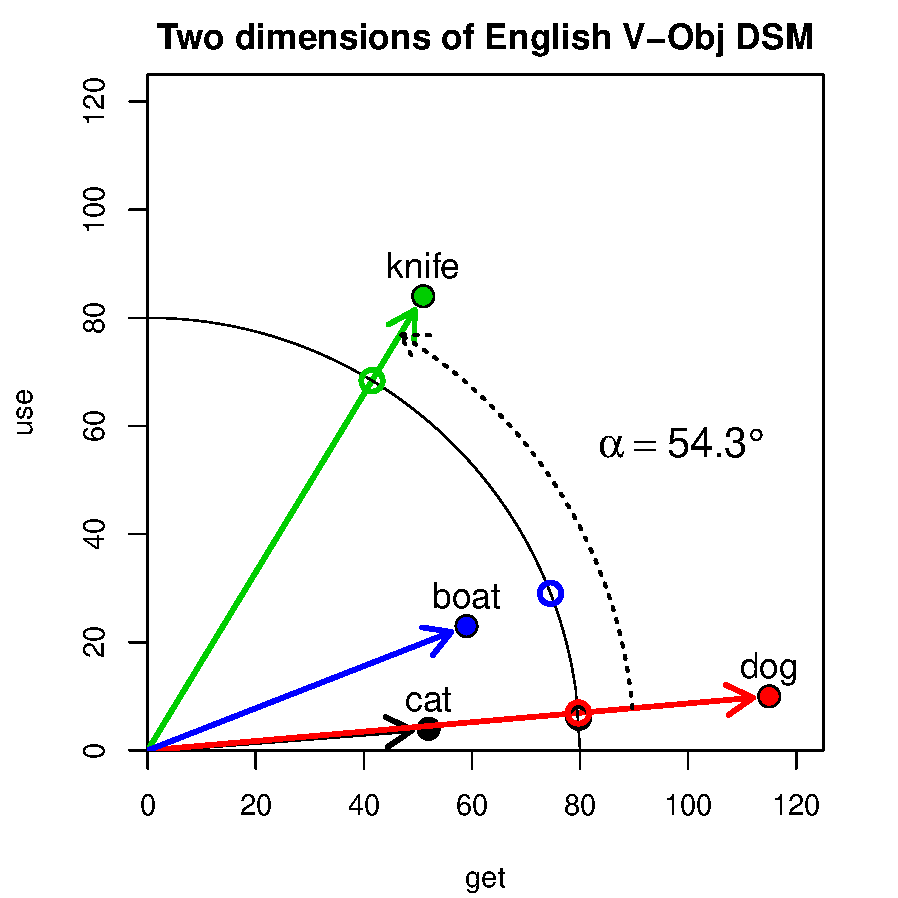
\includegraphics[width=6cm]{img/hieroglyph_2d_5}
    \end{column}
  \end{columns}
\end{frame}

\begin{frame}
  \frametitle{Overview of DSM parameters}
  % \framesubtitle{}

  \ungap[1]
  \begin{center}
    Linguistic pre-processing (definition of terms)\\
    $\Downarrow$\\
    Term-context \vs\ term-term matrix\\
    $\Downarrow$\\
    Size \& type of context / structured \vs\ unstructered\\
    $\Downarrow$\\
    Geometric \vs\ probabilistic interpretation\\
    $\Downarrow$\\
    Feature scaling\\
    $\Downarrow$\\
    Normalisation of rows and/or columns\\
    $\Downarrow$\\
    Similarity / distance measure\\
    $\Downarrow$\\
    \h{Compression}
  \end{center}
\end{frame}

\begin{frame}
  \frametitle{Model compression = dimensionality reduction}
  % \framesubtitle{}

  \begin{itemize}
  \item Co-occurrence matrix $\mathbf{M}$ is often unmanageably large\\
    and can be extremely sparse
    \begin{itemize}
    \item Google Web1T5: 1M $\times$ 1M matrix with one trillion
      cells, of which less than 0.05\% contain nonzero counts \citep{Evert:10a}
    \end{itemize}
  \item[\So] Compress matrix by reducing dimensionality (= rows)
    \begin{itemize}
    \item[]\pause
    \end{itemize}
  \item \h{Feature selection}: columns with high frequency \& variance
    \begin{itemize}
    \item measured by entropy, chi-squared test, \ldots
    \item may select correlated (\so uninformative) dimensions
    \item joint selection of multiple features is expensive
    \end{itemize}
    \pause
  \item \h{Projection} into (linear) subspace
    \begin{itemize}
    \item principal component analysis (PCA)
    \item independent component analysis (ICA)
    \item random indexing (RI)
    \item[\hand] intuition: preserve distances between data points
    \end{itemize}
  \end{itemize}
\end{frame}

\begin{frame}
  \frametitle{Dimensionality reduction \& latent dimensions}
  %% \framesubtitle{}

  \citet{Landauer:Dumais:97} claim that LSA dimensionality reduction (and related PCA technique) uncovers \h{latent dimensions} by exploiting correlations between features.

  \begin{columns}
    \begin{column}{6.5cm}
      \begin{itemize}
      \item Example: term-term matrix
      \item V-Obj cooc's extracted from BNC
        \begin{itemize}
        \item targets = noun lemmas\\
        \item features = verb lemmas
        \end{itemize}
      \item feature scaling: association scores (modified $\log$ Dice
        coefficient)
      \item $k=111$ nouns with $f \geq 20$\\
        (must have non-zero row vectors)
      \item $n=2$ dimensions: \emph{buy} and \emph{sell}
      \end{itemize}
    \end{column}
    \begin{column}{4cm}
      \begin{center}\footnotesize
        \begin{tabular}{l|rr}
          noun & \emph{buy} & \emph{sell} \\
          \hline
          \emph{bond}      &  0.28 &  0.77\\
          \emph{cigarette} & -0.52 &  0.44\\
          \emph{dress}     &  0.51 & -1.30\\
          \emph{freehold}  & -0.01 & -0.08\\
          \emph{land}      &  1.13 &  1.54\\
          \emph{number}    & -1.05 & -1.02\\
          \emph{per}       & -0.35 & -0.16\\
          \emph{pub}       & -0.08 & -1.30\\
          \emph{share}     &  1.92 &  1.99\\
          \emph{system}    & -1.63 & -0.70
        \end{tabular}
      \end{center}
    \end{column}
  \end{columns}
\end{frame}

\begin{frame}[c]
  \frametitle{Dimensionality reduction \& latent dimensions}
  %% \framesubtitle{}
  \begin{center}
    \ungap[1]
    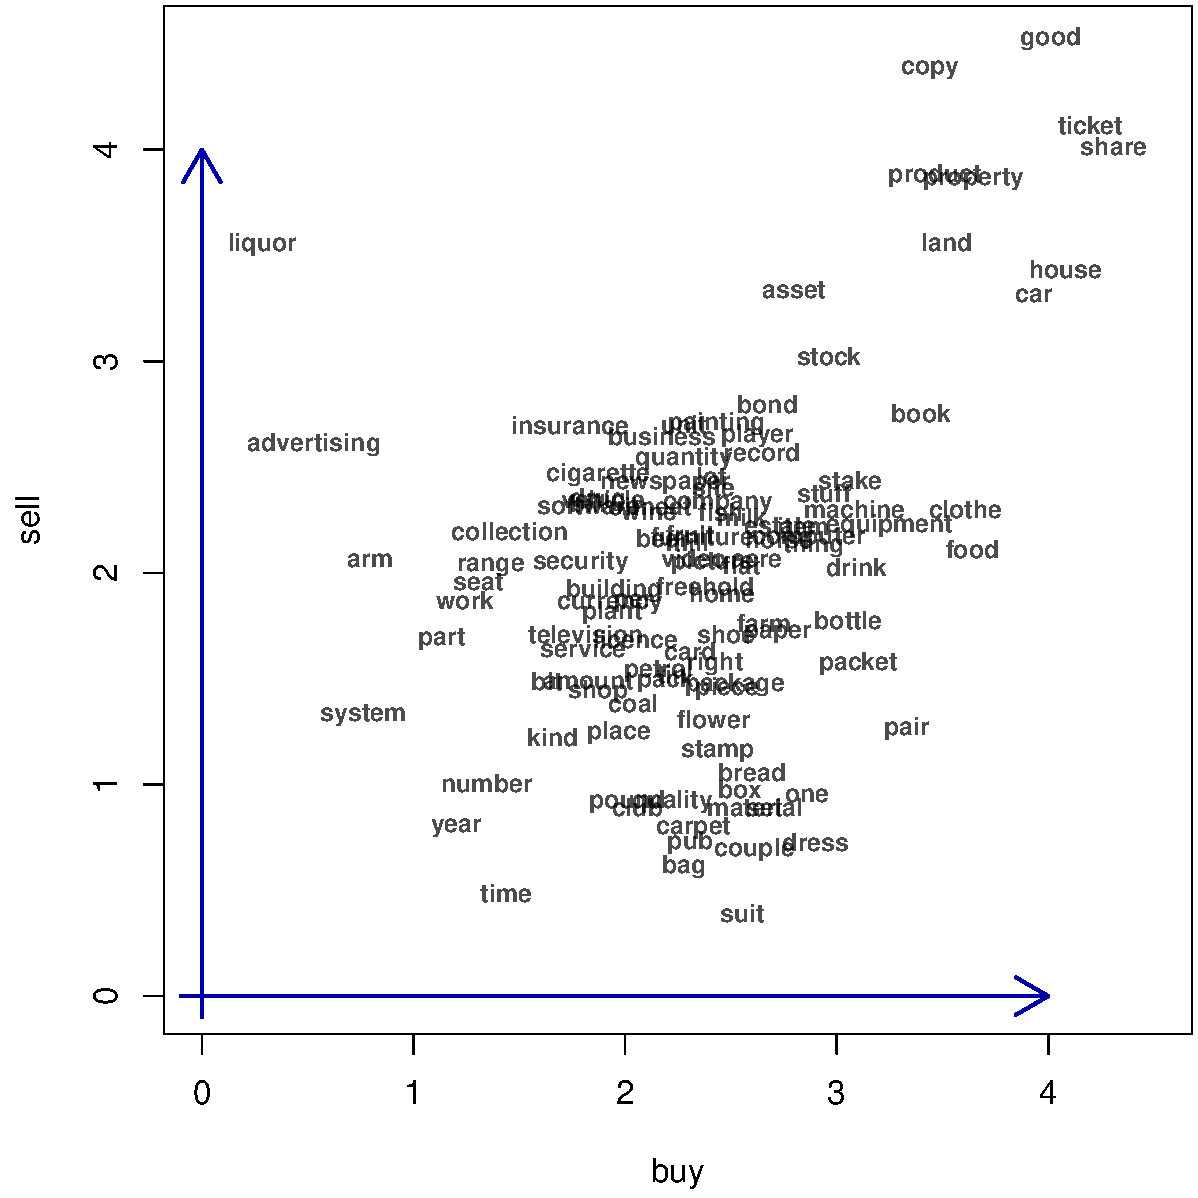
\includegraphics[width=8cm]{img/3_buy_sell_labels_only}
  \end{center}
\end{frame}

\begin{frame}
  \frametitle{Motivating latent dimensions \& subspace projection}
  %% \framesubtitle{}

  \begin{itemize}
  \item The \h{latent property} of being a commodity is ``expressed''
    through associations with several verbs: \emph{sell}, \emph{buy},
    \emph{acquire}, \ldots
  \item Consequence: these DSM dimensions will be \h{correlated}
  \item[]\pause
  \item Identify \h{latent dimension} by looking for strong correlations\\
    (or weaker correlations between large sets of features)%
  \item Projection into subspace $V$ of $k < n$ latent dimensions\\
    as a ``\h{noise reduction}'' technique \so \hh{LSA}
  \item Assumptions of this approach:
    \begin{itemize}
    \item ``latent'' distances in $V$ are semantically meaningful
    \item other ``residual'' dimensions represent chance co-occurrence
      patterns, often particular to the corpus underlying the DSM
    \end{itemize}
  \end{itemize}
\end{frame}

\begin{frame}[c]
  \frametitle{The latent ``commodity'' dimension}
  %% \framesubtitle{}
  \begin{center}
    \ungap[1]
    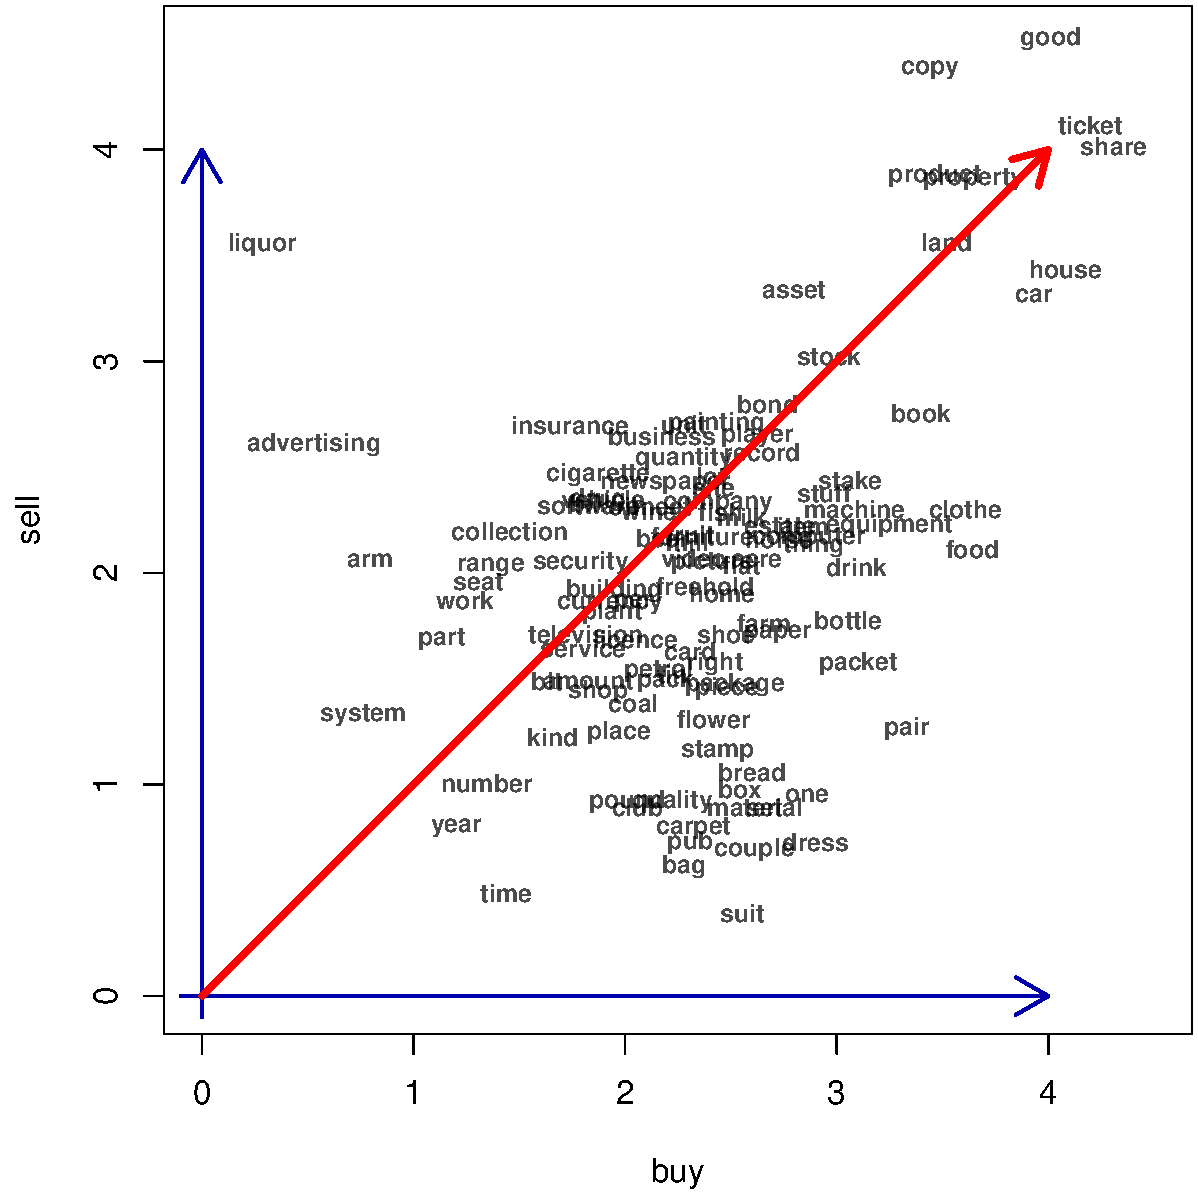
\includegraphics[width=8cm]{img/3_buy_sell_labels_latent}
  \end{center}
\end{frame}


%%%%%%%%%%%%%%%%%%%%%%%%%%%%%%%%%%%%%%%%%%
\subsection{Examples}

\begin{frame}
  \frametitle{Some well-known DSM examples}

  \ungap
  \begin{block} {Latent Semantic Analysis \citep{Landauer:Dumais:97}}
  \begin{itemize}
  \item term-context matrix with document context
  \item weighting: log term frequency and term entropy
  \item distance measure: cosine
  \item compression: SVD
  \end{itemize}
  \end{block}
 
 \begin{block} {Hyperspace Analogue to Language \citep{Lund:Burgess:96}}
  \begin{itemize}
  \item term-term matrix with surface context
  \item structured (left/right) and distance-weighted frequency counts
  \item distance measure: Minkowski metric ($1\leq p \leq 2$)
  \item compression: feature selection (high variance)
  \end{itemize}
  \end{block}
\end{frame}

\begin{frame}
  \frametitle{Some well-known DSM examples}

  \ungap
  \begin{block} {Infomap NLP \citep{Widdows:04}}
  \begin{itemize}
  \item term-term matrix with unstructured surface context
  \item weighting: none
  \item distance measure: cosine
  \item compression: SVD
  \end{itemize}
  \end{block}
 
  \begin{block} {Random Indexing (Karlgren \& Sahlgren 2001)}
    \begin{itemize}
    \item term-term matrix with unstructured surface context
    \item weighting: various methods 
    \item distance measure: various methods
    \item compression: random indexing (RI)
    \end{itemize}
  \end{block}
\end{frame}

\begin{frame}
  \frametitle{Some well-known DSM examples}

  \ungap
  \begin{block}{Dependency Vectors \citep{Pado:Lapata:07}}
  \begin{itemize}
  \item term-term matrix with unstructured dependency context
  \item weighting: log-likelihood ratio
  \item distance measure: information-theoretic \citep{Lin:98a}
  \item compression: none
  \end{itemize}
  \end{block}
 
 \begin{block} {Distributional Memory  (Baroni \& Lenci 2009)}
  \begin{itemize}
  \item both term-context and term-term matrices
  \item context: structured dependency context
  \item weighting: local-MI association measure
  \item distance measure: cosine
  \item compression: none
  \end{itemize}
  \end{block}
 \end{frame}


%%% Local Variables: 
%%% mode: latex
%%% TeX-master: "../workspace"
%%% End: 

%%%%%%%%%%%%%%%%%%%%%%%%%%%%%%%%%%%%%%%%%%%%%%%%%%%%%%%%%%%%%%%%%%%%%%
\section{Usage and evaluation of DSM}

%%%%%%%%%%%%%%%%%%%%%%%%%%%%%%%%%%%%%%%%%%
\subsection{What to do with DSM distances}

\begin{frame}
  \frametitle{Nearest neighbours}
  \framesubtitle{DSM based on verb-object relations from BNC, reduced to 100 dim.\ with SVD}
  % \framesubtitle{}

  Neighbours of \h{dog} (cosine angle):
  \begin{itemize}\item[\hand]
    girl (45.5), boy (46.7), horse(47.0), wife (48.8), baby (51.9),
    daughter (53.1), side (54.9), mother (55.6), boat (55.7),
    rest (56.3), night (56.7), cat (56.8), son (57.0), man (58.2), 
    place (58.4), husband (58.5), thing (58.8), friend (59.6), \ldots
  \end{itemize}

  \gap
  Neighbours of \h{school}:
  \begin{itemize}\item[\hand]
    country (49.3), church (52.1), hospital (53.1), house (54.4),
    hotel (55.1), industry (57.0), company (57.0), home (57.7), family
    (58.4), university (59.0), party (59.4), group (59.5), building
    (59.8), market (60.3), bank (60.4), business (60.9), area (61.4),
    department (61.6), club (62.7), town (63.3), library (63.3), 
    room (63.6), service (64.4), police (64.7), \ldots
  \end{itemize}
  \addnote{Neighbours and neighbourhood plots from BNC verb-object DSM, reduced to 100 dimensions by SVD.}%
\end{frame}

\begin{frame}[c]
  \frametitle{Nearest neighbours}
  % \framesubtitle{}

  \begin{center}
    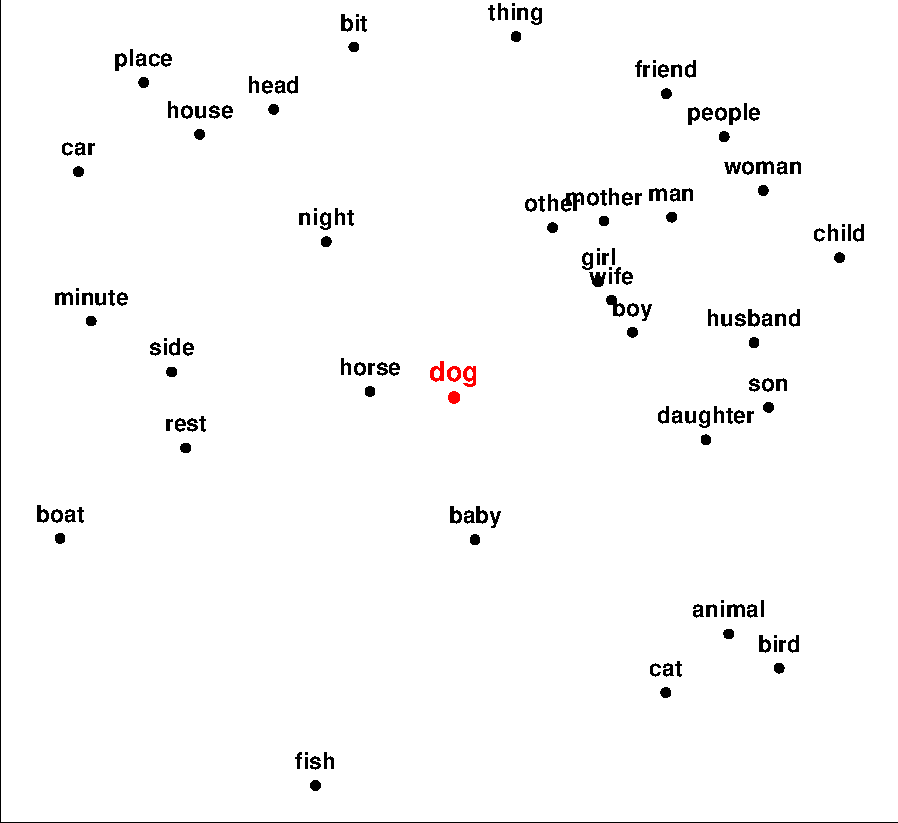
\includegraphics[width=8cm]{img/neighbourhood_dog}
  \end{center}
\end{frame}

\begin{frame}[c]
  \frametitle{Clustering}
  % \framesubtitle{}

  \begin{center}
    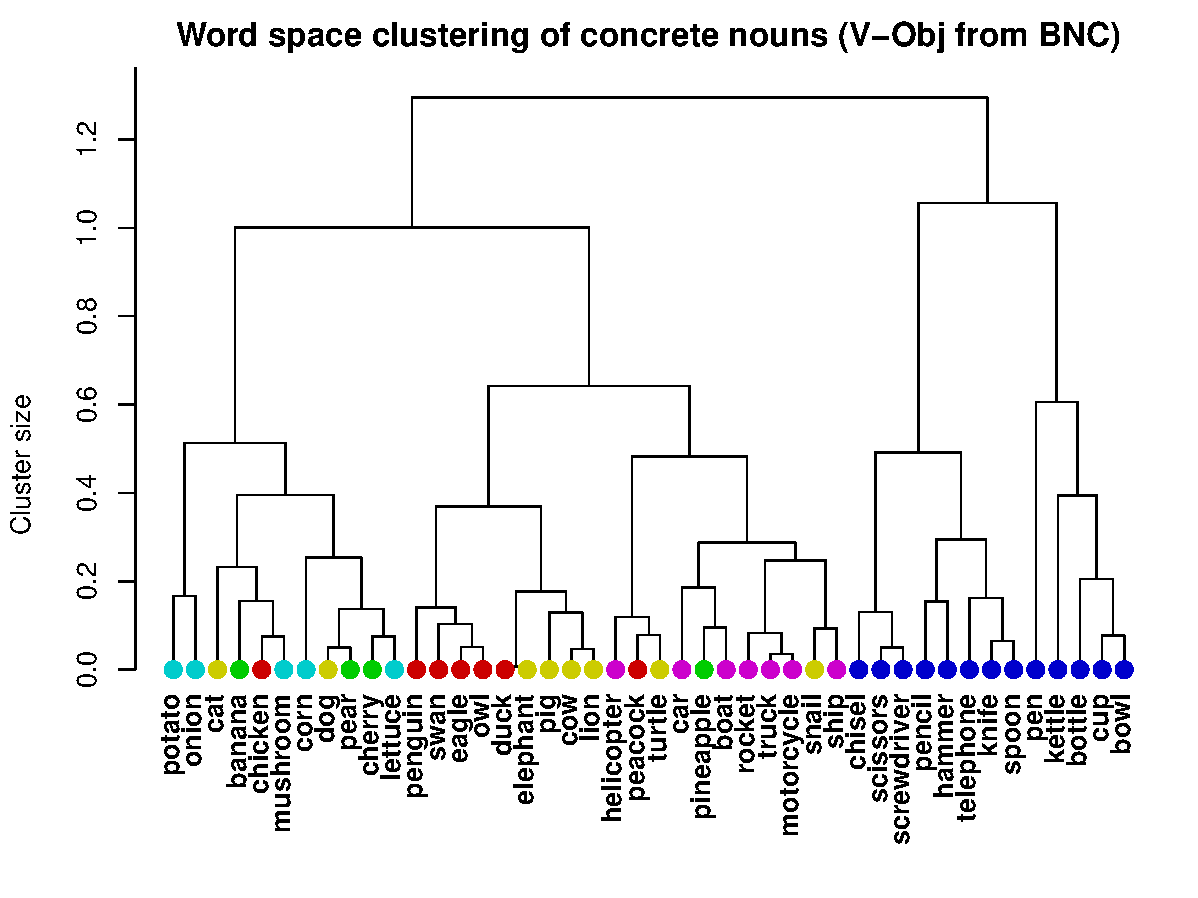
\includegraphics[width=100mm]{img/hieroglyph_clustering}
  \end{center}
\end{frame}

\begin{frame}[c]
  \frametitle{Semantic maps}
  % \framesubtitle{}

  \begin{center}
    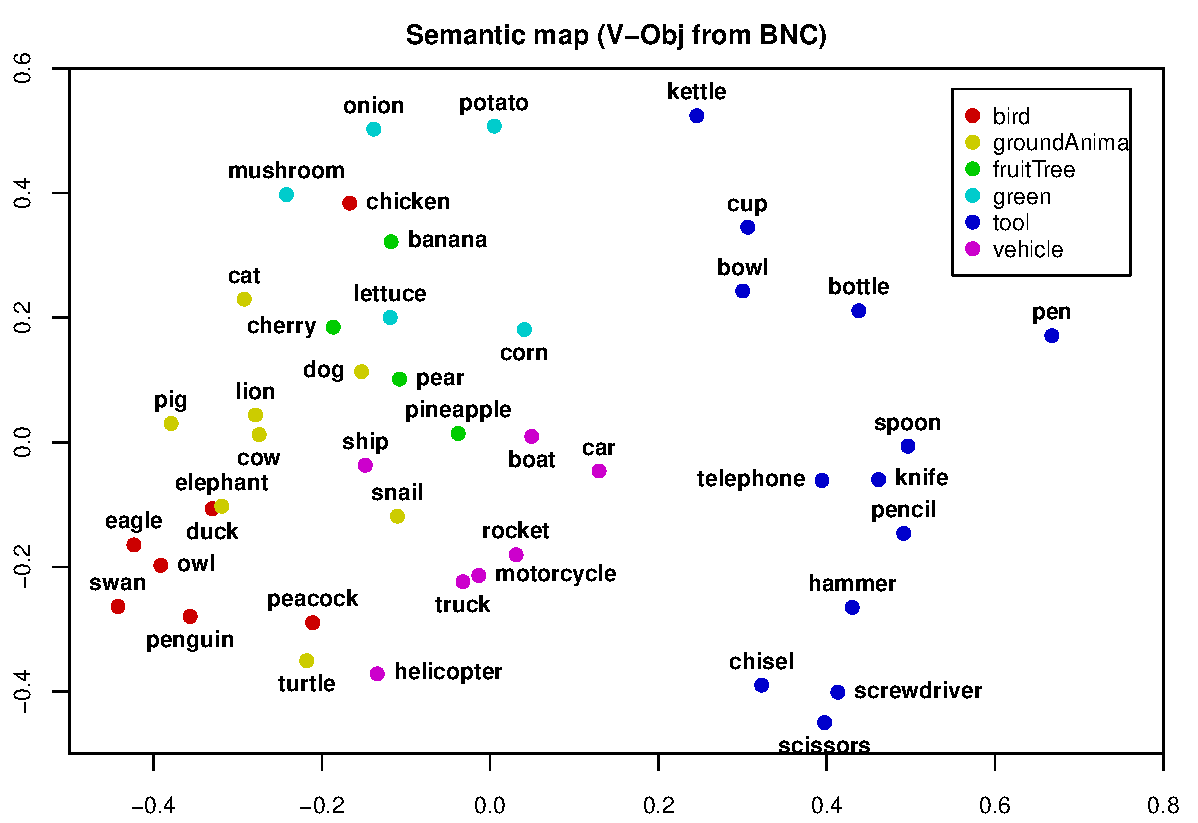
\includegraphics[width=100mm]{img/hieroglyph_semantic_map}
  \end{center}
\end{frame}

\begin{frame}[c]
  \frametitle{Latent dimensions}
  % \framesubtitle{}

  \begin{center}
    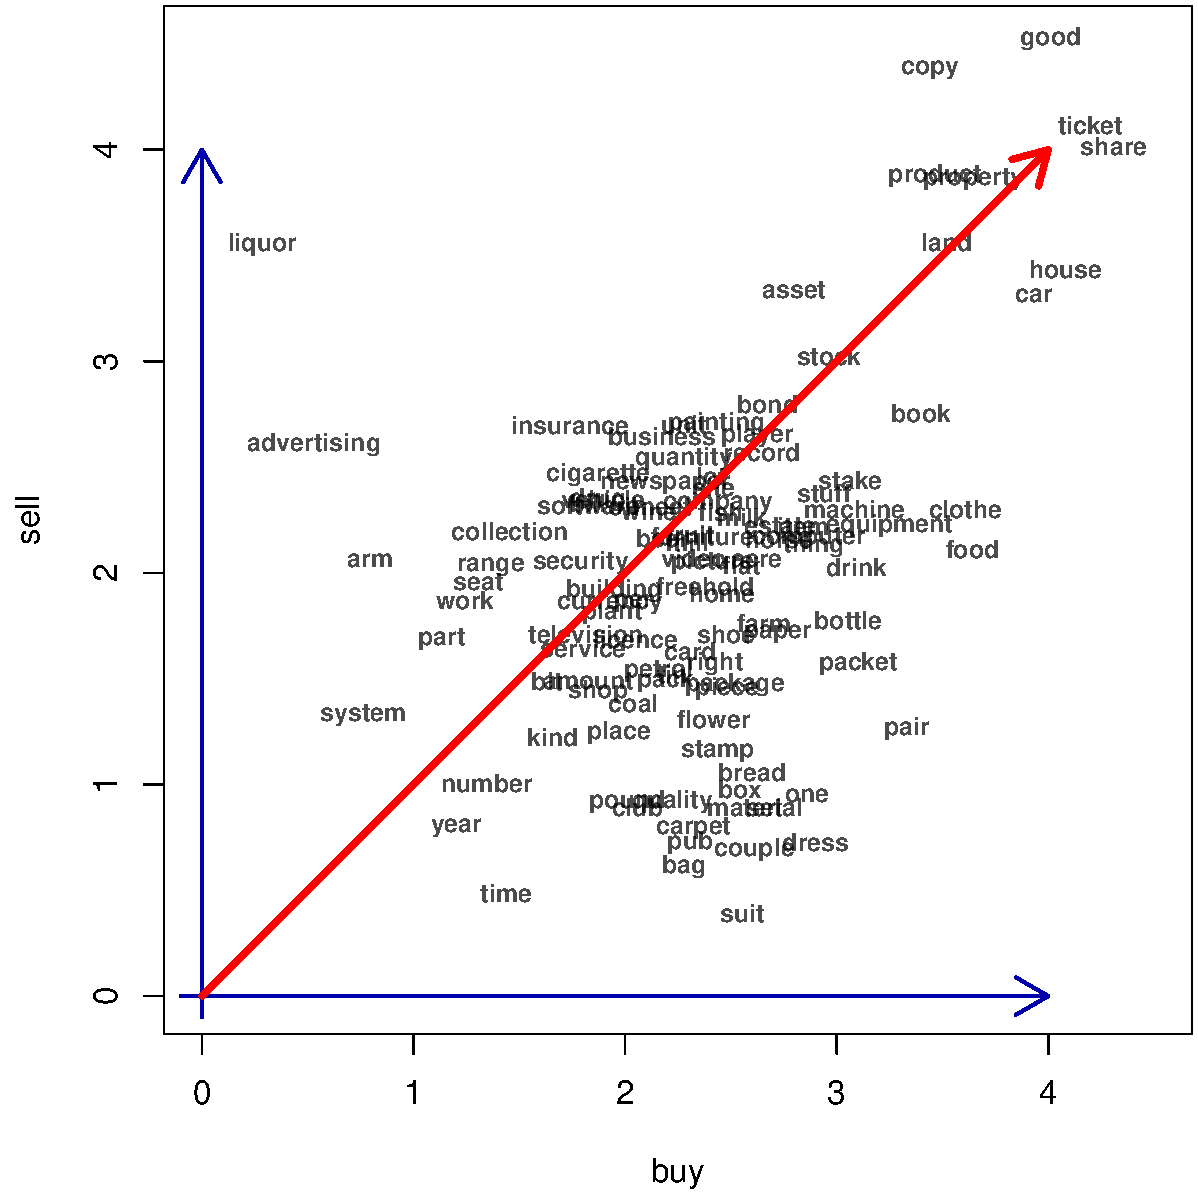
\includegraphics[width=8cm]{img/3_buy_sell_labels_latent}
  \end{center}
\end{frame}

\begin{frame}[c]
  \frametitle{Semantic similarity graph (topological structure)}
  % \framesubtitle{}

  \begin{center}
    \begin{tabular}{@{}cc@{}}
    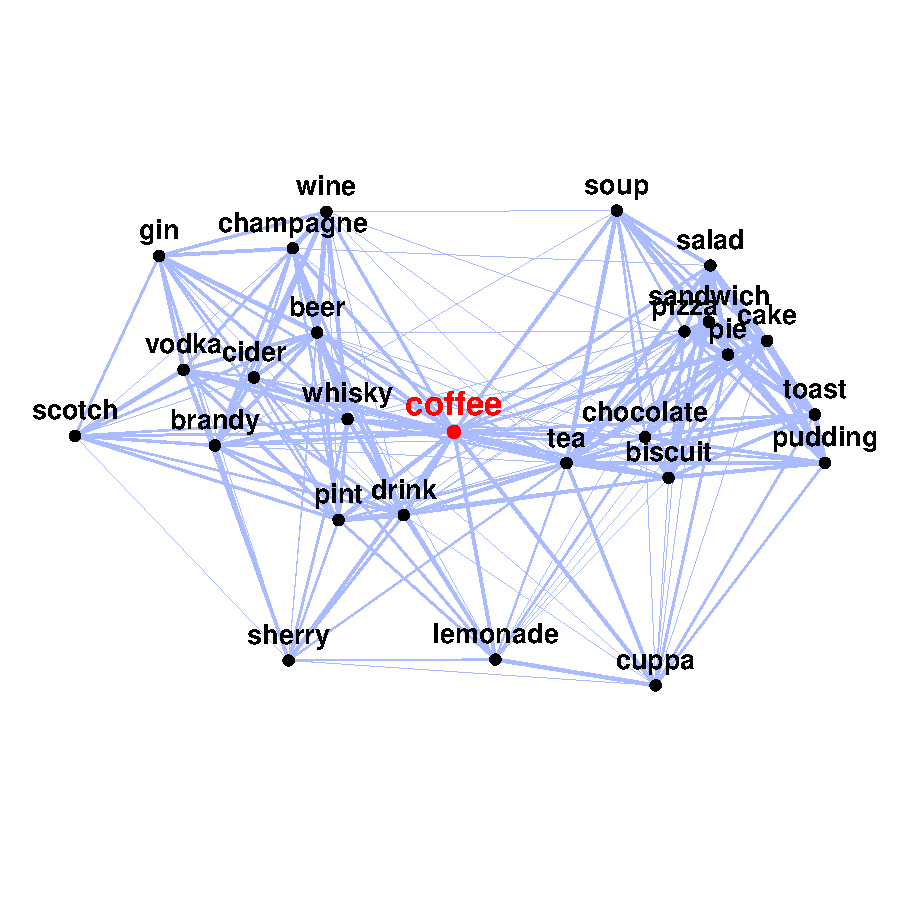
\includegraphics[width=55mm]{img/neighbourhood_coffee} &
    \visible<2->{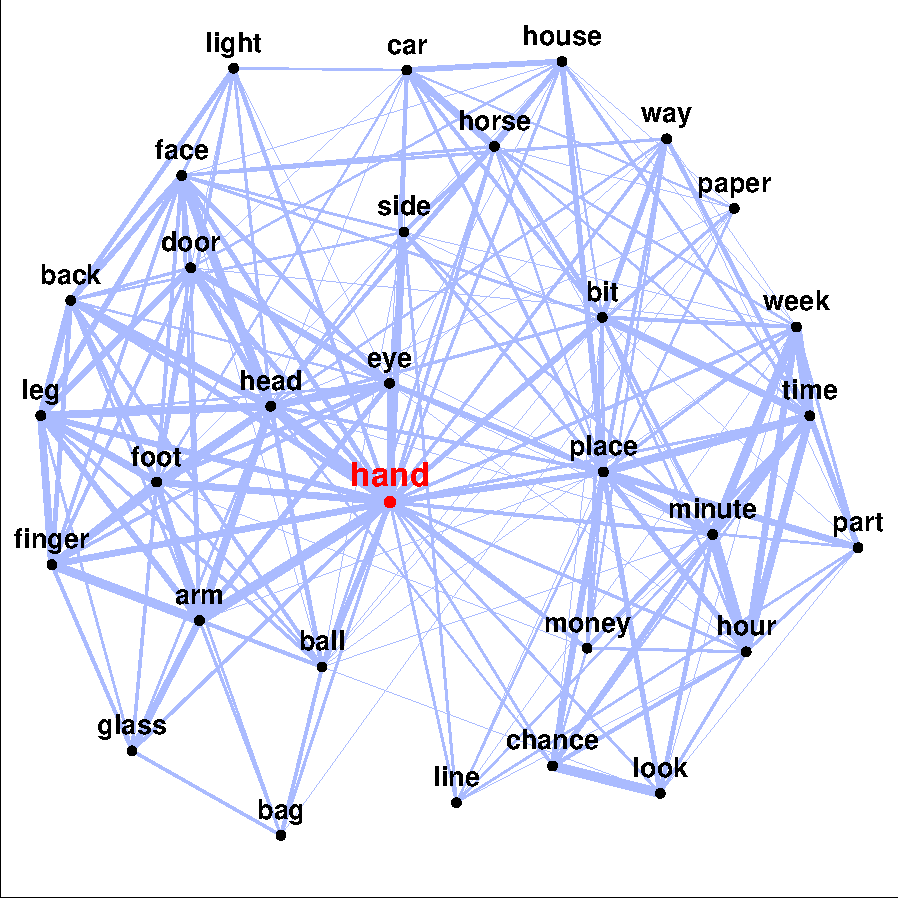
\includegraphics[width=55mm]{img/neighbourhood_hand}}
  \end{tabular}
  \end{center}
\end{frame}



%%%%%%%%%%%%%%%%%%%%%%%%%%%%%%%%%%%%%%%%%%
\subsection{Evaluation: semantic similarity and relatedness}

\begin{frame}
\frametitle{Distributional similarity as semantic similarity}

\begin{itemize}
\item DSMs interpret semantic similarity as a \primary{quantitative notion}
\begin{itemize}
\item if $\va$ is closer to $\vb$ than to $\Vector{c}$ in the distributional
vector space, then $a$ is more semantically similar to $b$ than to $c$
\end{itemize}
\end{itemize}

\begin{center}
  \begin{tabular}{l|l|l}
      \primary{rhino} & \primary{fall} & \primary{rock}\\
      \hline
      woodpecker&    rise&         lava\\
      rhinoceros&    increase&     sand\\
      swan&          fluctuation&  boulder\\
      whale&         drop&         ice\\
      ivory&         decrease&     jazz\\
      plover&        reduction&    slab\\
      elephant&      logarithm&    cliff\\
      bear&          decline&      pop\\
      satin&         cut&          basalt\\
      sweatshirt&    hike&         crevice\\
    \end{tabular}
  \end{center}
\end{frame}


\begin{frame}
\frametitle{Types of semantic relations in DSMs}

\begin{itemize}
\item Neighbors in DSMs have different types of
\primary{semantic relations}
\end{itemize}

\ungap[1.5]\footnotesize
 \begin{columns}[t]
    \column{.5\textwidth}
    \begin{block}{\emph{car} {\small (InfomapNLP on BNC; n = 2)}}
      \begin{itemize}
      \item  van {\color{counterpoint} co-hyponym}
      \item vehicle {\color{counterpoint} hyperonym}
      \item truck {\color{counterpoint} co-hyponym}
      \item motorcycle {\color{counterpoint} co-hyponym}
      \item driver {\color{counterpoint} related entity}
      \item motor {\color{counterpoint} part}
      \item lorry {\color{counterpoint} co-hyponym}
      \item motorist {\color{counterpoint} related entity}
      \item cavalier {\color{counterpoint} hyponym}
      \item bike {\color{counterpoint} co-hyponym}
\end{itemize}
\end{block}
\column{.5\textwidth}
\begin{block} {\emph{car} {\small (InfomapNLP on BNC; n = 30)}}
  \begin{itemize}
  \item drive {\color{counterpoint} function}
  \item park {\color{counterpoint} typical action}
  \item bonnet {\color{counterpoint} part}
  \item windscreen {\color{counterpoint} part}
  \item hatchback {\color{counterpoint} part}
\item headlight {\color{counterpoint} part}
\item jaguar {\color{counterpoint} hyponym}
\item garage {\color{counterpoint} location}
\item cavalier {\color{counterpoint} hyponym}
\item tyre {\color{counterpoint} part}
\end{itemize}
\end{block}
  \end{columns}

\end{frame}


\begin{frame}
\frametitle{Semantic similarity and relatedness}

\begin{itemize}
\item \primary{Semantic similarity} - two words sharing a high 
number of  salient features (attributes)
\begin{itemize}
\item synonymy (\emph{car/automobile})
\item hyperonymy (\emph{car/vehicle)}
\item co-hyponymy (\emph{car/van/truck})
\end{itemize}
\pause
\item \primary{Semantic relatedness} (Budanitsky \& Hirst 2006) - two words semantically
associated without being necessarily similar
\begin{itemize}
\item function (\emph{car/drive})
\item meronymy (\emph{car/tyre})
\item location (\emph{car/road})
\item attribute (\emph{car/fast})
\end{itemize}
\end{itemize}
\end{frame}

%%%%%%%%%%%%%%%%%%%%%%%%%%%%%%%%%%%%%%%%%%
\subsection{Attributional similarity}

\begin{frame}
  \frametitle{DSMs and semantic similarity}
  \begin{itemize}
   \item These models emphasize \primary{paradigmatic} similarity
   \begin{itemize}
    \item words that tend to occur in the same contexts
    \end{itemize}
  \item Words that share many contexts will correspond to concepts
    that share many attributes (\primary{attributional similarity}),
    i.e. concepts that are \primary{taxonomically/ontologically similar}
    \begin{itemize}
    \item synonyms (\emph{rhino/rhinoceros})
    \item antonyms and values on a
      scale (\emph{good/bad})
      \item co-hyponyms (\emph{rock/jazz})
      \item hyper- and hyponyms (\emph{rock/basalt})
    \end{itemize}
  \item Taxonomic similarity is seen as the fundamental semantic
    relation, allowing categorization, generalization, inheritance
  \end{itemize}
\end{frame}



\begin{frame}
  \frametitle{Evaluation of attributional similarity}
  
  \begin{itemize}
  \item \primary{Synonym identification}
  \begin{itemize}
\item TOEFL test
\end{itemize}
  \item \primary{Modeling semantic similarity}
    judgments
   \begin{itemize}
\item the Rubenstein/Goodenough norms
\end{itemize}
  \item \primary{Noun categorization}
  \begin{itemize}
\item the ESSLLI 2008 dataset
\end{itemize}
  \item \primary{Semantic priming}
  \begin{itemize}
\item the Hodgson  dataset
\end{itemize}

  \end{itemize}
\end{frame}

%%%%%%%%%%%%%%%%%%%%%%%%%%%%%%%%%%%%%%%%%%
%\subsection{Synonym identification and semantic similarity judgements}


\begin{frame}\frametitle{The TOEFL synonym task}

  \begin{itemize}
  \item The TOEFL dataset
  \begin{itemize}
  \item<1-> 80 items
  \item<1-> Target: \emph{levied}\\
    Candidates:
    \emph{\alert<2->{imposed}, believed, requested, correlated}
    \end{itemize}
    \item[]
  \item<3-> DSMs and TOEFL
  \begin{enumerate}
\item take vectors of the target ($\Vector{t}$) and of the candidates
($\Vector{c}_1 \dots \Vector{c}_n$)
\item measure the distance between $\Vector{t}$ and $\Vector{c}_i$, with
$1 \leq i \leq n$ 
\item select $\Vector{c}_i$ with the shortest distance in space from $\Vector{t}$
\end{enumerate}
  \end{itemize}

\end{frame}


\begin{frame}
  \frametitle{Human performance on the synonym match task}

  \begin{itemize}
  \item Average foreign test taker: 64.5\%
  \item Macquarie University staff (Rapp 2004):
    \begin{itemize}
    \item Average of 5 non-natives: 86.75\%
    \item Average of 5 natives: 97.75\%
    \end{itemize}

  \end{itemize}

\end{frame}


\begin{frame}
  \frametitle{DSMs take the TOEFL}
  \begin{itemize}
  \item \primary{Humans}
    \begin{itemize}
    \item Foreign test takers: 64.5\%
    \item Macquarie non-natives: 86.75\%
    \item Macquarie natives: \primary{97.75\%}
    \end{itemize}
  \item \primary{Machines}
    \begin{itemize}
    \item Classic LSA: 64.4\%
    \item Padó and Lapata's dependency-based model: 73\%
    \item Rapp's 2003 SVD-based model trained on lemmatized BNC:
      \primary{92.5\%}
    \end{itemize}
  \end{itemize}
\end{frame}


\begin{frame}
\frametitle{Semantic similarity judgments}

  \begin{description}
  \item [ Dataset] Rubenstein and Goodenough (1965) (R\&G) of\\
 65 noun pairs rated by 51 subjects on a 0-4 scale
    \begin{center}
    \begin{tabular}{llr}
      \emph{car} & \emph{automobile} & \primary{3.9}\\
     \emph{food} &  \emph{fruit}  & \primary{2.7}\\
      \emph{cord} & \emph{smile} & \primary{0.0}\\
    \end{tabular}
      \end{center}
\end{description}
\pause
\begin{itemize}
\item DSMs \vs\ Rubenstein \& Goodenough
 \begin{enumerate}
\item for each test pair $(w_1, w_2)$, take vectors $\Vector{w}_1$ and $\Vector{w}_2$
\item measure the distance (e.g.\ cosine) between $\Vector{w}_1$ and $\Vector{w}_2$
\item measure (Pearson) correlation between vector distances and R\&G average judgments \citep{Pado:Lapata:07}
\end{enumerate}
\end{itemize}
\end{frame}  

\begin{frame}
\frametitle{Semantic similarity judgments: example}
\ungap[1]
\begin{center}
  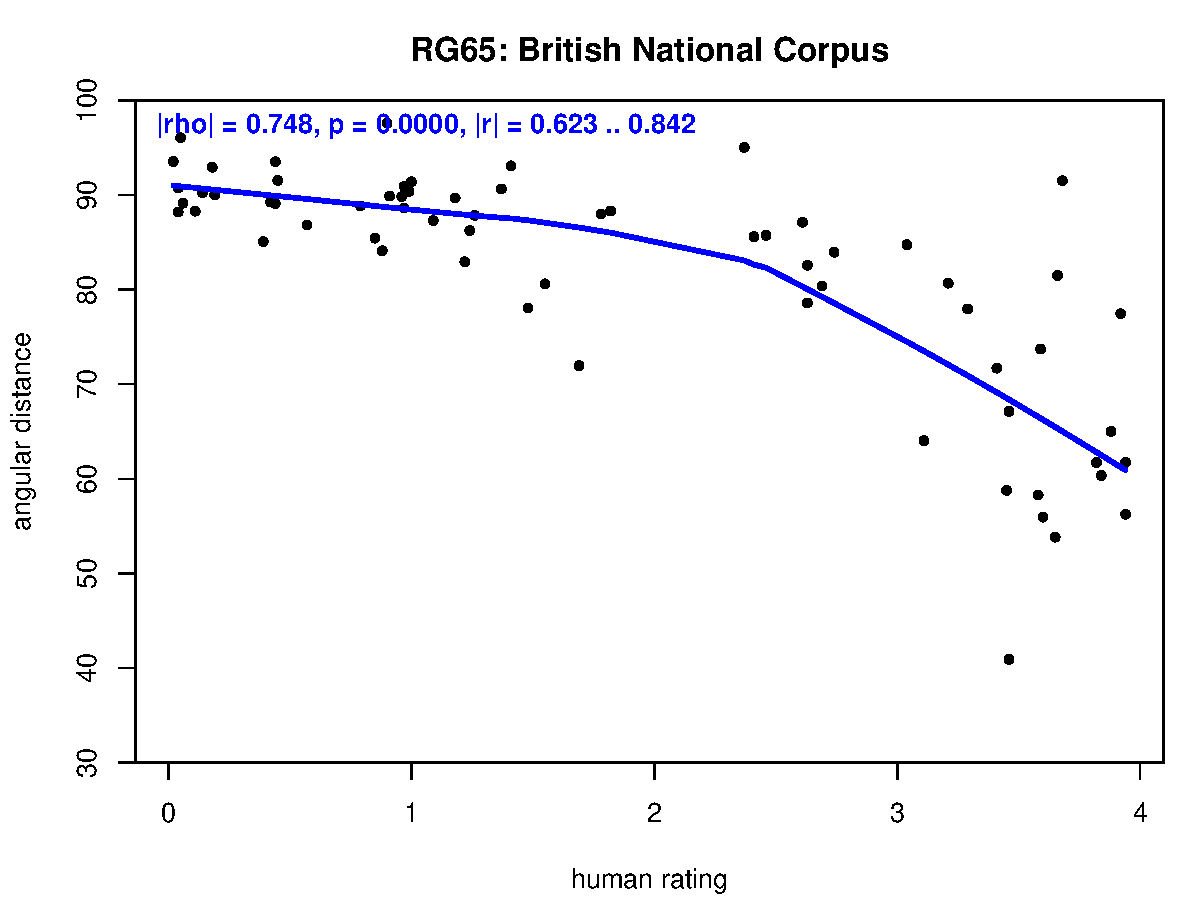
\includegraphics[width=9cm]{img/bnc_rg65}
\end{center}
\end{frame}

\begin{frame}
\frametitle{Semantic similarity judgments: results}
    \begin{center}
      \begin{tabular}{|l|r|}
      \hline
      \emph{model} & $r$\\
      \hline
      \hline
      dep-filtered+SVD & 0.8\\
      \hline
      dep-filtered    & 0.7\\
      \hline
      dep-linked  (DM) & 0.64\\
      \hline
      window & 0.63\\
      \hline
    \end{tabular}

    \gap[1]
    \primary{Results for RG65 task}
      \end{center}
\end{frame}


%%%%%%%%%%%%%%%%%%%%%%%%%%%%%%%%%%%%%%%%%%
%\subsection{Noun categorization}


\begin{frame}
\frametitle{Categorization}

\begin{itemize}
\item In \primary{categorization tasks}, subjects are typically asked to assign experimental items -- objects, images, words -- to a given category or group items belonging to the same category
\begin{itemize}
\item categorization requires an understanding of the relationship between the items in a category
\end {itemize}
\item Categorization is a basic cognitive operation presupposed by further semantic tasks
\begin{itemize}
\item \primary{inference}
\begin{itemize}
\item if X is a CAR then X is a VEHICLE
\end{itemize}
\item \primary{compositionality}
\begin{itemize}
\item $\lambda y:\text{FOOD}\; \lambda x:\text{ANIMATE}; eat(x,y)$
\end{itemize}
\end{itemize}
\item ``Chicken-and-egg'' problem for relationship of categorization and similarity (cf.\ Goodman 1972, Medin et al.\ 1993)
\end{itemize}
\end{frame}


\frame{
\frametitle{Noun categorization}

  \begin{description}
  \item [ Dataset] 44 concrete nouns (ESSLLI 2008 Shared Task)
   \begin{itemize}
  \item 24 natural entities
     \begin{itemize}
    \item 15 animals:\\
      7 birds (\emph{eagle}), 8 ground animals (\emph{lion})
    \item 9 plants: 4 fruits (\emph{banana}), 5 greens (\emph{onion})
    \end{itemize}
  \item 20 artifacts
    \begin{itemize}
    \item 13 tools (\emph{hammer}), 7 vehicles (\emph{car})
    \end{itemize}
  \end{itemize}
\end{description}
\pause

\begin{itemize}
\item DSMs and noun categorization
\begin{itemize}
\item categorization can be operationalized as a \primary{clustering task}
\begin{enumerate}
\item for each noun $w_i$ in the dataset, take its vector $\vw_i$
\item use a \primary{clustering method} to group close vectors $\vw_i$
\item evaluate whether clusters correspond to gold-standard semantic
  classes (purity, entropy, \ldots)
\end{enumerate}

\end{itemize}

\end{itemize}

}




\begin{frame}
\frametitle{Noun categorization}
\begin{itemize}
\item Clustering experiments with CLUTO (Karypis 2003)
\begin{itemize}
\item repeated bisection algorithm
\item 6-way (birds, ground animals, fruits, greens,
tools and vehicles), 3-way (animals, plants and
artifacts) and 2-way (natural and artificial entities) clusterings
\end{itemize}
\pause
\item Clusters evaluation
\begin{itemize}
\item \primary{entropy} -- whether words from different classes are represented in the same cluster (\primary{best = 0})
\item \primary{purity} -- degree to which a cluster contains words from one class only (\primary{best = 1})
\item \primary{global score} across the three clustering experiments
\begin{displaymath}
\sum_{i=1}^3 \text{Purity}_i -  \sum_{i=1}^3 \text{Entropy}_i
\end{displaymath}

\end{itemize}
\end{itemize}
\end{frame}


\begin{frame}
\frametitle{Noun categorization: example}
\ungap[1]
\begin{center}
  \only<beamer:1| handout:0>{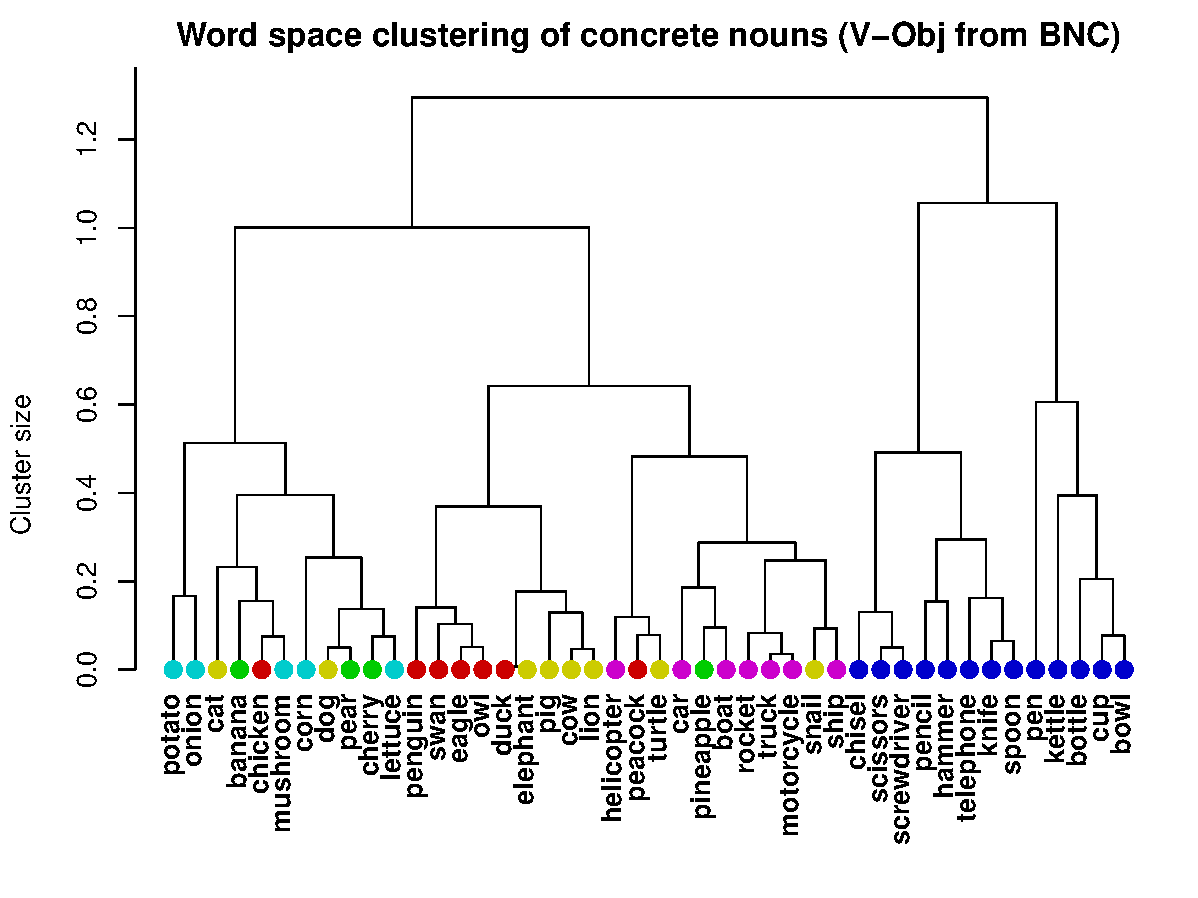
\includegraphics[width=8cm]{img/hieroglyph_clustering}}%
  \only<beamer:2-| handout:1>{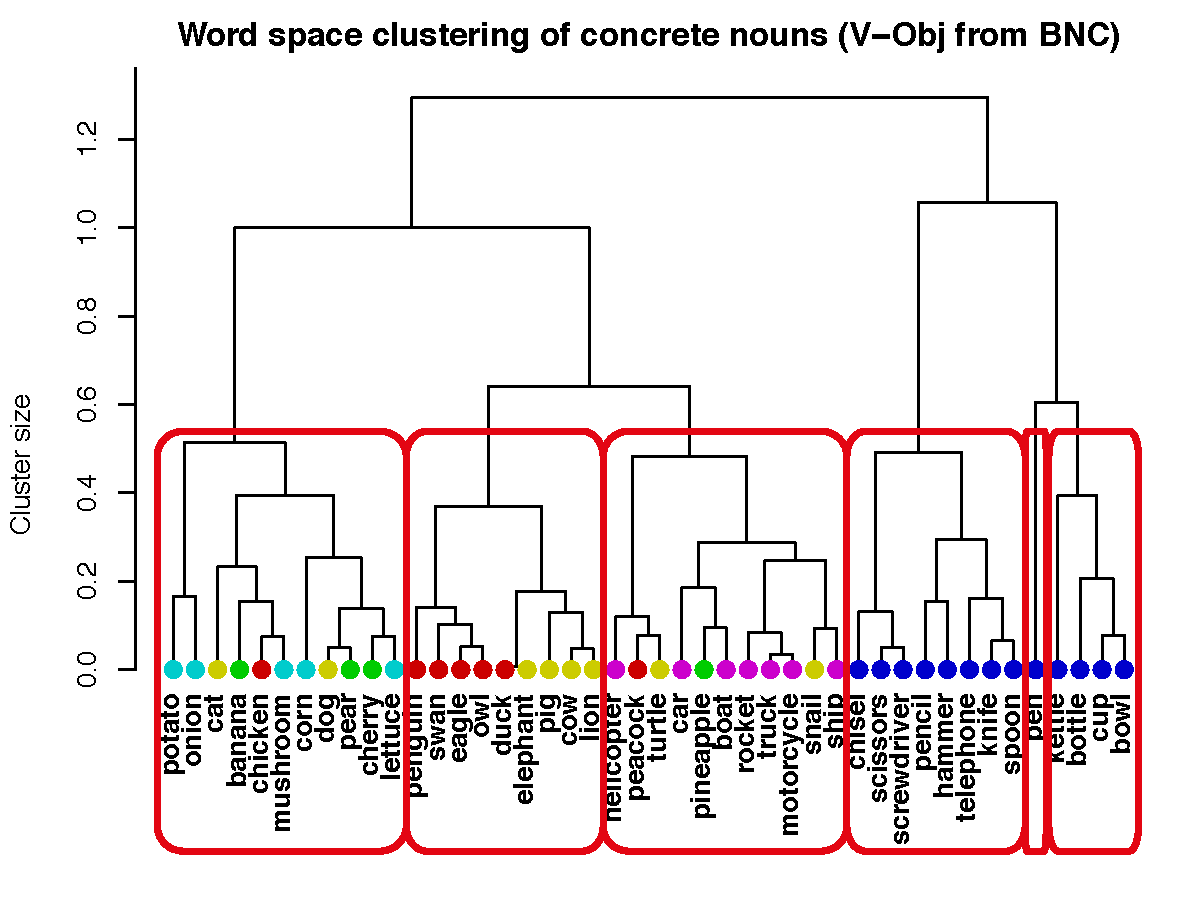
\includegraphics[width=8cm]{img/hieroglyph_clustering_6}}%
\end{center}
\ungap[1]
\begin{itemize}
\item<3-> majority labels: greens, birds, vehicles, tools, tools, tools
\item<3-> correct: 5/11, 5/9, 6/11, 8/8, 1/1, 4/4
\item<4-> purity = 30 correct out of 44 = 68.2\%
\end{itemize}

\end{frame}


\frame{
\frametitle{Noun categorization: results}

 \begin{center}
  \begin{tabular}{|l|r|r||r|r||r|r||r|}
      \hline
      \emph{model} &\multicolumn{2}{|c||}{\emph{6-way}} &  \multicolumn{2}{|c||}{\emph{3-way}} & \multicolumn{2}{|c||}{\emph{2-way}}&  \multicolumn{1}{|c|}{\emph{global}}\\
      \cline{2-7}
      &   \emph{P} & \emph{E}  & \emph{P} & \emph{E}  & \emph{P} & \emph{E} &\\
      \hline
      \hline
      Katrenko & 89 & 13 & 100 & 0 & 80 & 59 & 197\\ 
      \hline
      Peirsman+ & 82 & 23 & 84 & 34 & 86 & 55 & 140\\
      \hline
      dep-typed (DM) & 77 & 24 & 79 & 38 & 59 & 97 & 56\\
      \hline
      dep-filtered & 80 &28 & 75& 51& 61& 95 & 42\\
      \hline
      window & 75& 27&  68& 51& 68& 89   &44\\
      \hline
      Peirsman$-$ & 73 & 28 & 71 & 54 & 61 & 96 & 27\\
      \hline
      Shaoul & 41& 77& 52& 84 & 55& 93& -106\\
      \hline
    \end{tabular}
\end{center}

\begin{center}\footnotesize
  {\tt Katrenko, Peirsman+/-, Shaoul}: ESSLLI 2008 Shared Task\\
  {\tt DM}: Baroni \& Lenci (2009)
\end{center}
     
 
}


%%%%%%%%%%%%%%%%%%%%%%%%%%%%%%%%%%%%%%%%%%\
%\subsection{Semantic priming}

\begin{frame}
  \frametitle{Semantic priming}
  \begin{itemize}
  \item Hearing/reading a ``related'' prime facilitates access to a
    target in various lexical tasks (naming, lexical decision,
    reading)
    \begin{itemize}
  \item  the word \emph{pear} is recognized/accessed faster if it is
    heard/read after \emph{apple}
    \end{itemize}
    \pause
  \item Hodgson (1991) single word lexical decision task, 136
    prime-target pairs (cf.\ Padó \& Lapata 2007)
    \begin{itemize}
  \item similar amounts of priming for different
    semantic relations between primes and targets (approx.~23 pairs
    per relation):
    \begin{itemize}
    \item synonyms (synonym): \emph{to dread/to fear}
    \item antonyms (antonym): \emph{short/tall}
    \item coordinates (coord): \emph{train/truck}
    \item super- and subordinate pairs (supersub): \emph{container/bottle}
    \item free association pairs (freeass): \emph{dove/peace}
    \item phrasal associates (phrasacc): \emph{vacant/building}
    \end{itemize}
  \end{itemize}
\end{itemize}
\end{frame}



\begin{frame}
  \frametitle{Simulating semantic priming}
  \framesubtitle{McDonald \& Brew (2004), Padó \& Lapata (2007)}
 \begin{itemize}
 \item DSMs and semantic priming
  \begin{enumerate}
  \item for each related prime-target pair, 
  measure cosine-based similarity between pair items (e.g.,
    \emph{to dread/to fear})
    \pause
  \item to estimate \primary{unrelated primes}, take average of cosine-based similarity of target with other
    primes from same relation data-set (e.g., \emph{value/to fear})
    \pause
  \item similarity between related items should be significantly higher
    than average similarity between unrelated items
    \item[]
  \end{enumerate}
  \pause
\item Significant effects ($p < .01$) for all semantic relations 
  \begin{itemize}
  \item strongest effects for synonyms, antonyms \& coordinates
  \end{itemize}
  \end{itemize}
\end{frame}


%%%%%%%%%%%%%%%%%%%%%%%%%%%%%%%%%%%%%%%%%%\
\subsection{Relational similarity}


\begin{frame}
  \frametitle{Finding and distinguishing semantic relations}
  \begin{itemize}
  \item Classic distributional semantic models are based on
    \primary{attributional} similarity
    \begin{itemize}
    \item single words/concepts that share attributes / tend to occur
      in the same contexts are semantically similar
    \end{itemize}
  \item Attributional similarity can be modeled with DSMs that have \primary{single words}
  as matrix rows
  \begin{itemize}
  \item matrix columns represent attributes shared by similar words
\end{itemize}
  \end{itemize}
  \pause
   \begin{center}
   \begin{tabular}{l|c|c|c}

         &{\color{counterpoint}die}           &{\color{counterpoint}kill}           &{\color{counterpoint}gun} \\
\hline
{\color{blue}teacher}  &109.4         &0.0             &0.0  \\
{\color{blue}victim}   &1335.2        &22.4            &0.0 \\
{\color{blue}soldier}  &4547.5        &1306.9        &105.9\\
{\color{blue}policeman} &68.6          &38.2           &30.5\\

  \end{tabular}
  \end{center}

  
  
\end{frame}


\begin{frame}
  \frametitle{Attributional and relational similarity}
  \framesubtitle{Turney (2006)}

  \begin{itemize}
  \item \emph{Policeman} is \primary{attributionally} similar to
    \emph{soldier}
    \begin{itemize}
    \item both occur in contexts like:
    \emph{kill X}, \emph{with gun}, \emph{for security}
    \end{itemize}
    \pause
  \item The pair \emph{policeman-gun} is \primary{relationally}
    similar to \emph{teacher-book}
    \begin{itemize}
    \item both are often connected by \emph{with}, \emph{use},
      \emph{of} in context
    \end{itemize}
    \pause
    \item It is not always possible to reduce relational similarity to attributional similarity
    \begin{itemize}
\item \emph{mason}:\emph{stone} :: \emph{carpenter}:\emph{wood}\\
  \vs\ \emph{traffic}:\emph{street} :: \emph{water}:\emph{riverbed}
\begin{itemize}
\item \emph{mason} - \emph{carpenter} and \emph{stone} - \emph{wood} are attributionally similar
\item \emph{traffic} - \emph{water} and \emph{street} - \emph{riverbed} are \primary{not} attributionally similar
\end{itemize}
\end{itemize}

  \end{itemize}
\end{frame}



\begin{frame}
  \frametitle{Finding and distinguishing semantic relations with DSMs}

  \begin{itemize}
    \item Find non-taxonomic semantic relations
      \begin{itemize}
      \item look at direct co-occurrences of \primary{word pairs} in texts (when
        we talk about a concept, we are likely to also mention its
        parts, function, etc.)
      \end{itemize}
      \pause
    \item Distinguish between different semantic relations
      \begin{itemize}
      \item use the contexts of pairs to measure pair similarity, and
        group them into coherent relation types by their contexts
      \item \emph{pairs} that occur in similar contexts (i.e.\
   \primary{connected by similar words and structures}) will tend to be
    related, with the shared contexts acting as a cue to the nature of
    their relation, i.e., measuring their \emph{relational} similarity
    (Turney 2006)
     
      \end{itemize}
  \end{itemize}
\end{frame}


\begin{frame}
  \frametitle{DSMs and relational similarity}
  
 \begin{description}
    \item [rows] \primary{word pairs}
    \item [columns] \primary{syntagmatic links} between the word pairs
    \end{description}

  \begin{center}
        \begin{tabular}{ll|c|c|c|c}
          &        &{\color{counterpoint}in}     &{\color{counterpoint}at}    &{\color{counterpoint}with}&{\color{counterpoint}use}  \\
          \hline
          {\color{secondary}teacher}&{\color{primary}school}  &11894.4&7020.1&28.9 &0.0 \\
          {\color{secondary}teacher}&{\color{primary}handbook}&2.5    &0.0   &3.2  &10.1\\
          {\color{secondary}soldier}&{\color{primary}gun}     &2.8    &10.3  &105.9&41.0\\
        \end{tabular}
      \end{center}
\end{frame}


\begin{frame}
  \frametitle{Recognizing SAT analogies}
    
  \begin{itemize}
\item 374 SAT multiple-choice questions (Turney 2006)
\item Each question  includes 1 target pair (stem) and 5 answer pairs
\item the task is to choose the pair most \emph{analogous} to the stem
  \begin{center}
  \begin{tabular}{ll}
    {\color{secondary}mason} & {\color{secondary}stone}\\
    \hline
    teacher & chalk\\
    \h<2->{carpenter} & \h<2->{wood}\\
    soldier & gun\\
    photograph & camera\\
    book & word\\
  \end{tabular}
  \end{center}
\item<3-> Relational analogue to the TOEFL task
\begin{enumerate}
\item <4-> for each pair $p$, take its row vector $\Vector{p}$
\item <5-> for each stem-pair, select the closest answer-pair\\
  (e.g.\ the one with the highest cosine similarity)
\end{enumerate}
\end{itemize}  
\end{frame}


\begin{frame}
  \frametitle{Recognizing SAT analogies: results}

\begin{center}
 \begin{table}[tbh]
  \begin{small}
    \begin{center}
      \begin{tabular}{|l|r||l|r|}
        \hline
        \emph{model} & \emph{\% correct} & \emph{model} & \emph{\% correct} \\
        \hline
        \hline
        LRA & 56.1&KnowBest & 43.0\\
        \hline
        PERT & 53.3& DM$-$ & 42.3\\
        \hline
        PairClass & 52.1&LSA& 42.0\\
        \hline
        VSM & 47.1&AttrMax & 35.0\\
        \hline
        DM+ & 45.3&AttrAvg & 31.0\\
        \hline
        PairSpace & 44.9&AttrMin & 27.3\\
        \hline
        \emph{k}-means & 44.0&\color{primary}{Random} & \color{primary}{20.0}\\
        \hline
      \end{tabular}
         \end{center}
  \end{small}
\end{table}
  \end{center}


 \begin{center}
  \footnotesize
  {\tt LRA, PERT, PairClass, VSM, KnowBest, LSA}: ACLWiki\\
  {\tt AttrMax, AttrAvg, AttrMin}: Turney(2006)\\
  {\tt DM+, DM-}: Baroni \& Lenci (2009)
\end{center}

\end{frame}

\begin{frame}
  \frametitle{Domain analogies}

  \begin{itemize}
  \item Turney (2008) extends the relational approach to entire
    analogical \emph{domains}
    \begin{center}
      \begin{tabular}{lll}
        solar system&$\rightarrow$& atom \\
        sun&$\rightarrow$& nucleus \\
        planet&$\rightarrow$& electron \\
        mass&$\rightarrow$& charge \\
        attracts&$\rightarrow$& attracts \\
        revolves&$\rightarrow$& revolves \\
        gravity&$\rightarrow$& electromagnetism \\
      \end{tabular}
    \end{center}
\end{itemize}
\end{frame}


\begin{frame}[c]
  \begin{center}
    \textcite{\LARGE Intermission}

    \gap[2]
    Time for a cup of coffee \ldots
  \end{center}
\end{frame}


%%% Local Variables: 
%%% mode: latex
%%% TeX-master: "../workspace"
%%% End: 



%%%%%%%%%%%%%%%%%%%%%%%%%%%%%%%%%%%%%%%%%%%%%%%%%%%%%%%%%%%%%%%%%%%%%%
%% References (if any)

\frame[allowframebreaks]{
  \frametitle{References}
  \bibliographystyle{natbib-stefan}
  \begin{scriptsize}
    \bibliography{dsm}
  \end{scriptsize}
}

\end{document}
